%%%%%%%%%%%%%%%%%%%%%%%%%%%%%%%%%%%%%%%%%%%%%%%%%%%%%%%%%%%%%%%%%%%%%%%%
% Template adapted from latex-mimosis:
% https://github.com/Pseudomanifold/latex-mimosis
%
% Copyright (c) 2022 Antonio Coín
%
% This work is licensed under a
% Creative Commons Attribution-ShareAlike 4.0 International License.
%
% You should have received a copy of the license along with this
% work. If not, see <http://creativecommons.org/licenses/by-sa/4.0/>.
%%%%%%%%%%%%%%%%%%%%%%%%%%%%%%%%%%%%%%%%%%%%%%%%%%%%%%%%%%%%%%%%%%%%%%%%


\documentclass{mimosis}

% Relative paths
\newcommand{\thesisPath}{chapters}

% Misc. packages
\usepackage{metalogo}
\usepackage{etoolbox}
\usepackage{tocloft}
%\usepackage{pdfpages}
\usepackage{placeins}
\usepackage{xcolor}
\usepackage{cancel}
\usepackage{bbding}

% Licensing
\usepackage[
    type={CC},
    modifier={by-sa},
    version={4.0},
]{doclicense}

% Make chapter number show in arabic
\renewcommand\cftchappresnum{\normalfont}

%% Primary color
\newcommand{\titlecolor}{teal}

% Large number and color for chapter
\renewcommand*{\chapterformat}{%
  \fontsize{60}{65}\selectfont\color{\titlecolor}\(\thechapter\)\autodot\enskip
}

%
% Colour for section numbers
%
\renewcommand*{\sectionformat}{%
  \textcolor{\titlecolor}{\(\thesection\)}\autodot\enskip%
}

%
% Colour for subsection numbers
%
\renewcommand*{\subsectionformat}{%
  \textcolor{\titlecolor}{\(\thesubsection\)}\autodot\enskip%
}

%
% Colour for subsubsection numbers
%
\renewcommand*{\subsubsectionformat}{%
  \textcolor{\titlecolor}{\(\thesubsubsection\)}\autodot\enskip%
}

%%%%%%%%%%%%%%%%%%%%%%%%%%%%%%%%%%%%%%%%%%%%%%%%%%%%%%%%%%%%%%%%%%%%%%%%
% Custom commands
%%%%%%%%%%%%%%%%%%%%%%%%%%%%%%%%%%%%%%%%%%%%%%%%%%%%%%%%%%%%%%%%%%%%%%%%

%% Math operators
\DeclareMathOperator*\argmin{arg\,min}
\DeclareMathOperator\supp{supp}
\DeclareMathOperator\Cov{Cov}
\DeclareMathOperator\Var{Var}

%% Math symbols
\newcommand{\N} {\ensuremath{\mathds{N}}}
\newcommand{\R} {\ensuremath{\mathds{R}}}
\newcommand{\E} {\ensuremath{\mathds{E}}}
\newcommand{\I} {\ensuremath{\mathds{I}}}
\renewcommand{\P} {\ensuremath{\mathds{P}}}

\newcommand{\D} {\ensuremath{\mathcal{D}}}
\newcommand{\X} {\ensuremath{\mathcal{X}}}
\newcommand{\K} {\ensuremath{\mathcal{K}}}
\newcommand{\T} {\ensuremath{\mathcal{T}}}
\newcommand{\U} {\ensuremath{\mathcal{U}}}
\newcommand{\Lcal} {\ensuremath{\mathcal{L}}}
\newcommand{\Hcal} {\ensuremath\mathcal{H}}

%% Better overline
\newcommand{\overbar}[1]{\mkern 1.5mu\overline{\mkern-1.5mu#1\mkern-1.5mu}\mkern 1.5mu}

%% Scalar product
\newcommand\dotprod[2]{\left\langle #1, #2 \right\rangle}

%%%%%%%%%%%%%%%%%%%%%%%%%%%%%%%%%%%%%%%%%%%%%%%%%%%%%%%%%%%%%%%%%%%%%%%%
% Hyperlinks, bookmarks and tables
%%%%%%%%%%%%%%%%%%%%%%%%%%%%%%%%%%%%%%%%%%%%%%%%%%%%%%%%%%%%%%%%%%%%%%%%

\definecolor{webgreen}{rgb}{0,0.5,0}
\usepackage[%
  colorlinks = true,
  citecolor  = teal, %webgreen,
  linkcolor  = teal, % RoyalBlue,
  urlcolor   = RoyalBlue,
  unicode,
  ]{hyperref}

\usepackage{bookmark}

% Space between rows in tables
\renewcommand{\arraystretch}{1.2}

%%%%%%%%%%%%%%%%%%%%%%%%%%%%%%%%%%%%%%%%%%%%%%%%%%%%%%%%%%%%%%%%%%%%%%%%
% Bibliography
%%%%%%%%%%%%%%%%%%%%%%%%%%%%%%%%%%%%%%%%%%%%%%%%%%%%%%%%%%%%%%%%%%%%%%%%

\usepackage[%
  autocite     = plain,
  backend      = biber,
  natbib       = true,
  doi          = false,
  url          = false,
  isbn         = false,
  giveninits   = true,
  hyperref     = true,
  maxbibnames  = 99,
  maxcitenames = 2,
  mincitenames = 1,
  uniquelist   = false,
  dashed       = false,
  sortcites    = true,
  style        = authoryear-comp,
  backref      = true
  ]{biblatex}


% Format references as {last-name}, {first-name-initials}
\DeclareNameAlias{sortname}{family-given}

% Volume number in parenthesis
\renewbibmacro*{volume+number+eid}{%
  \printfield{volume}%
%  \setunit*{\adddot}% DELETED
  \setunit*{\addnbthinspace}% NEW (optional); there's also \addnbthinspace
  \printfield{number}%
  \setunit{\addcomma\space}%
  \printfield{eid}}
\DeclareFieldFormat[article]{number}{\mkbibparens{#1}}

\addbibresource{bibliography.bib}

%%%
% Math Environments
%%%

\theoremstyle{theorem}
\newtheorem{theorem}{Theorem}[chapter]
\newtheorem{corollary}[theorem]{Corollary}
\newtheorem{lemma}[theorem]{Lemma}
\newtheorem{proposition}[theorem]{Proposition}

\theoremstyle{definition}
\newtheorem{definition}[theorem]{Definition}
\newtheorem{example}[theorem]{Example}

\theoremstyle{remark}
\newtheorem{remark}{Remark}

%%%
% Lists and footnotes
%%%

% Lists
\usepackage[shortlabels]{enumitem}
%\setlist{itemsep=0.05em}
\setlist{noitemsep}
\setlist[1]{labelindent=\parindent} % < Usually a good idea
\setlist[enumerate,1]{label=(\roman*)}

% Continuous counter for footnotes and figures
\counterwithout{footnote}{chapter}
\counterwithout{figure}{chapter}

%%%%%%%%%%%%%%%%%%%%%%%%%%%%%%%%%%%%%%%%%%%%%%%%%%%%%%%%%%%%%%%%%%%%%%%%
% Fonts
%%%%%%%%%%%%%%%%%%%%%%%%%%%%%%%%%%%%%%%%%%%%%%%%%%%%%%%%%%%%%%%%%%%%%%%%

\ifxetexorluatex
  \usepackage{unicode-math}
  \setmainfont{EB Garamond}
  %\setmathfont{latinmodern-math.otf}
  %\setmathfont[range={\mathcal,\mathbfcal}]{Garamond-Math.otf}
  \setmathfont{Libertinus Math}
  \setmathfont[range={\forall}]{Garamond-Math.otf}
  %\setmathfont{Garamond-Math.otf}
  \setmonofont[Scale=MatchLowercase]{Source Code Pro}
\else
  \usepackage[lf]{ebgaramond}
  \usepackage[oldstyle,scale=0.7]{sourcecodepro}
  \singlespacing
\fi

%%%%%%%%%%%%%%%%%%%%%%%%%%%%%%%%%%%%%%%%%%%%%%%%%%%%%%%%%%%%%%%%%%%%%%%%
% Incipit
%%%%%%%%%%%%%%%%%%%%%%%%%%%%%%%%%%%%%%%%%%%%%%%%%%%%%%%%%%%%%%%%%%%%%%%%

\title{\textbf{Bayesian RKHS-based methods in functional regression}}
\author{Antonio Coín Castro}

\begin{document}

\frontmatter
  % Titlepage

\begin{titlepage}
  \vspace*{5cm}
  \makeatletter
  \begin{center}
    \begin{singlespace*}
    \begin{Huge}
      \@title
    \end{Huge}\\[1cm]
    %
    \begin{large}
      Master's thesis
    \end{large}
    %
    \vskip 0.1cm
    \emph{by}
    \vskip 0.18cm
    \begin{Large}
    \textsc{\@author}
  \end{Large}
  \end{singlespace*}
        %
    \vfill

    Under the supervision of
    \begin{large}
    \vskip 0.1cm
    José\,Ramón\,Berrendero\,Díaz\\
    Antonio\,Cuevas\,González\\[1cm]
  \end{large}

    A document submitted in partial fulfillment
    of the requirements for the\\
    \emph{Master's degree in Data Science}\\
    at\\
    \textsc{Universidad Autónoma de Madrid}\\[1cm]

    Madrid, 2022
  \end{center}
  \makeatother
\end{titlepage}
\newpage


%\thispagestyle{empty}
%\null
%\newpage



\thispagestyle{empty}
%\renewcommand*{\chapterpagestyle}{empty}
\pagebreak
\hspace{0pt}
%\vspace{17cm}
\vfill
\begin{center}
    \begin{minipage}[t]{12.5cm}
        \doclicenseThis
        The \LaTeX\ source code for this document is openly available at \texttt{\url{https://www.github.com/antcc/tfm}}, while the Python source code for the experiments carried out is available at \texttt{\url{https://www.github.com/antcc/rk-bfr}}.
    \end{minipage}
\end{center}
\vfill
\hspace{0pt}
\pagebreak
\newpage

%\thispagestyle{empty}
%\null
%\newpage

  %%%%%%%%%%%%%%%%%%%%%%%%%%%%%%%%%%%%%%%%%%%%%%%%%%%%%%%%%%%%%%%%%%%%%%%%
% Copyright (c) 2022 Antonio Coín
%
% This work is licensed under a
% Creative Commons Attribution-ShareAlike 4.0 International License.
%
% You should have received a copy of the license along with this
% work. If not, see <http://creativecommons.org/licenses/by-sa/4.0/>.
%%%%%%%%%%%%%%%%%%%%%%%%%%%%%%%%%%%%%%%%%%%%%%%%%%%%%%%%%%%%%%%%%%%%%%%%

%%%%%%%%%%%%%%%%%%%%%%%%%%%%%%%%%%%%%%%%%%%%%%%%%%%%%%%%%%%%%%%%%%%%%%%%
\begin{center}
  \begin{Large}
  \textsc{Abstract}
\end{Large}
\end{center}
%%%%%%%%%%%%%%%%%%%%%%%%%%%%%%%%%%%%%%%%%%%%%%%%%%%%%%%%%%%%%%%%%%%%%%%%

\noindent This work is framed within the field of Functional Data Analysis, a branch of statistics in which the objects of interest are random functions in a functional space instead of, say, random points in \(\R^p\). Due to the infinite-dimensional nature of the data, the most common \(L^2\)-models for functional linear and logistic regression present some complications that require further simplifications, usually in the form of regularization or dimensionality reduction.

We propose a novel Bayesian approach for functional linear and logistic regression models based on the theory of reproducing kernel Hilbert spaces (RKHS's). These recently-proposed models build upon the RKHS associated with the covariance function of the underlying stochastic process, and can be viewed as a finite-dimensional approximation to the classical functional regression paradigm. The corresponding functional model (or the functional logistic equation in the case of binary response) is determined by a function living on a dense subspace of the RKHS of interest, which has a tractable parametric form. By imposing a suitable prior distribution on this space, we can perform data-driven inference via standard Bayes methodology. The posterior distribution can be estimated through Markov chain Monte Carlo methods, which do not require a complete specification of the posterior density.

We derive several prediction strategies from the approximate posterior distribution, including a Bayesian-motivated variable selection procedure. We show through a comprehensive set of experiments that these methods are competitive against other usual alternatives in terms of predictive performance, both in simulated examples and real data sets. Overall, our proposed model is simple with regard to interpretation and implementation, and has an added flexibility thanks to the ambient Bayesian framework.\\

\noindent
\textsc{keywords:} functional data, linear regression, logistic regression, reproducing kernel Hilbert space, Bayesian inference, Markov chain Monte Carlo.


  %\newgeometry{top=1.75cm, bottom=5cm}
  \vspace*{-1.8cm}
  \tableofcontents
  %\restoregeometry

\mainmatter

%%%%%%%%%%%%%%%%%%%%%%%%%%%%%%%%%%%%%%%%%%%%%%%%%%%%%%%%%%%%%%%%%%%%%%%%
% Copyright (c) 2022 Antonio Coín
%
% This work is licensed under a
% Creative Commons Attribution-ShareAlike 4.0 International License.
%
% You should have received a copy of the license along with this
% work. If not, see <http://creativecommons.org/licenses/by-sa/4.0/>.
%%%%%%%%%%%%%%%%%%%%%%%%%%%%%%%%%%%%%%%%%%%%%%%%%%%%%%%%%%%%%%%%%%%%%%%%

%%%%%%%%%%%%%%%%%%%%%%%%%%%%%%%%%%%%%%%%%%%%%%%%%%%%%%%%%%%%%%%%%%%%%%%%
\chapter{Introduction}\label{ch:introduction}
%%%%%%%%%%%%%%%%%%%%%%%%%%%%%%%%%%%%%%%%%%%%%%%%%%%%%%%%%%%%%%%%%%%%%%%%

Over the last few decades, situations involving data in the form of functions have become commonplace in many statistical scenarios, as more and more information is available worldwide with an ever-increasing level of granularity in the measurements. In particular, functional data problems are far from unheard of in the data science and machine learning community, since they have attracted the attention of researchers and practitioners equally. Medical data, weather indicators or stock exchange indices are examples of elements that benefit from a functional treatment, where the observations are regarded as single entities rather than as a conglomerate of individual points.

Under a functional framework, the objects of interest are \textit{random functions} instead of random points in a finite-dimensional space. While in principle the functional data could be simply regarded as a discretized vector in a very high dimension (an indeed such a discretization is performed in practice), there are often many advantages in taking into account the functional nature of the data, ranging from modeling the possibly high correlation among points that are close in the domain, to extracting information that may be hidden in the derivatives of the function in question. Thus, the general idea is to assume the existence of an underlying sufficiently smooth function that generates each (possibly noisy) functional observation, even though we only record it on a finite grid of points.

To see what this kind of data looks like, Figure~\ref{fig:tecator_orig} shows an example of a functional data set, which is known in the literature as the Tecator data set, and whose elements represent near-infrared absorbance curves of meat samples. The objective here is to predict the fat content based on this absorbance spectrum, separating the samples into those with ``high'' and ``low'' fat content. At first glance it does not seem that the trajectories contain much relevant information to help classify the samples. However, after a suitable smoothing of the data (e.g. by representing each function in a Fourier basis) we can take the derivatives of the curves. In this case, after differentiating twice a clearer pattern emerges (see Figure~\ref{fig:tecator_derivatives}), one from which inference and prediction will surely be easier.

\begin{figure}[ht!]
  \begin{subfigure}[b]{0.48\textwidth}
    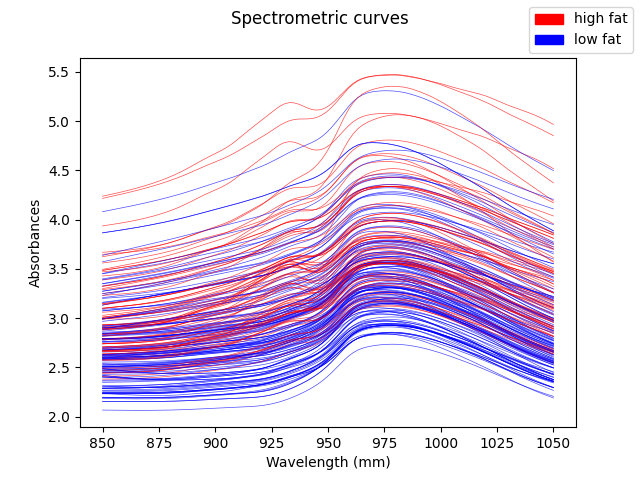
\includegraphics[width=\textwidth]{tecator}
    \caption{Original curves}\label{fig:tecator_orig}
  \end{subfigure}
  \hfill
  \begin{subfigure}[b]{0.48\textwidth}
    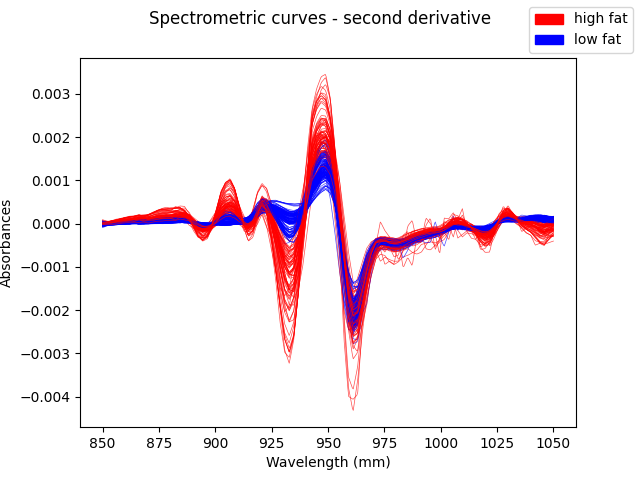
\includegraphics[width=\textwidth]{tecator_derivative}
    \caption{Second derivatives}\label{fig:tecator_derivatives}
  \end{subfigure}
  \caption{Curves in the Tecator data set and their second derivatives (after smoothing).}\label{fig:tecator}
\end{figure}

In recent years numerous proposals have arisen on how to suitably deal with functional data, all of them encompassed under the term Functional Data Analysis (FDA), which essentially explores statistical techniques to process, model and make inference on data varying over a continuum. A partial survey on such techniques and methods is \citet{cuevas2014partial}, while a more detailed exposition of the theory and applications can be found for example in \citet{ramsay2005functional}, \citet{hsing2015theoretical} or the book by \citet{horvath2012inference}. As the name suggests, FDA techniques are heavily inspired by functional analysis tools and methods: Hilbert spaces, orthonormal systems, linear operators, and so on. In particular, a notion that also intersects with the classical theory of machine learning and pattern recognition, and that has gained traction in recent years, is that of reproducing kernel Hilbert spaces (RKHS's). We will demonstrate throughout this work how these spaces of functions possess properties that allow for an efficient treatment of functional data.

On the other hand, Bayesian inference methods are ubiquitous in the realm of statistics, and their usual non-parametric approach also makes use of random functions, though in a slightly different manner than in the FDA context. However, the two methodologies can certainly interact and benefit from one another, as we intend to show in this thesis. We will be particularly interested in Markov chain Monte Carlo (MCMC) methods, which allow us to approximate an arbitrary posterior distribution through a function proportional to its density.

\begin{center}
\color{teal}\FourStar
\end{center}

In this work we are concerned with functional linear and logistic regression models, that is, situations where the goal is to predict a continuous or dichotomous variable from functional observations. Even though these problems can be formally stated with almost no differences from their finite-dimensional counterparts, there are some fundamental challenges as well as some subtle drawbacks that emerge as a result of working in infinite dimensions. Moreover, we will concentrate our efforts on the case in which the response is a scalar, though function-on-function and function-on-scalar regression are also interesting scenarios widely explored in the literature. To set a common framework, throughout this work we will consider a scalar response variable \(Y\) (either continuous or binary) which has some dependence on a stochastic \(L^2\)-process \(X=X(t)=X(t, \omega)\) with trajectories in \(L^2[0, 1]\) (i.e. a process with finite second moments and whose realizations are square-integrable functions indexed on \([0,1]\)). The underlying probability space \((\Omega, \mathcal A, \P)\) is not important. We will further suppose that \(X\) is centered, that is to say, its mean function \(m(t)=\E[X(t)]\) vanishes for all \(t\in[0,1]\). In addition, we will tacitly assume the existence of a \textit{labeled} data set \(\D_n =\{(x_i, y_i): i=1,\dots, n\}\) of independent observations from \((X, Y)\), where the functional observations are recorded on a common finite grid \(\{t_j\}\subset [0, 1]\). Our ultimate aim will be to accurately predict the response corresponding to unlabeled samples from \(X\). Figure~\ref{fig:linear_data_example} depicts a typical data set used in functional regression, and we already saw in Figure~\ref{fig:tecator} what a functional classification data set may look like.

\enlargethispage{1\baselineskip}

\begin{figure}[htbp!]
  \centering
  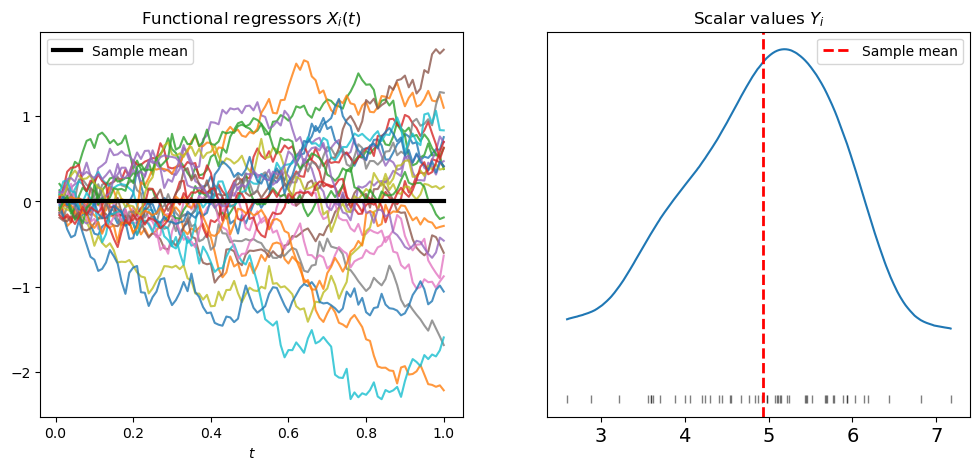
\includegraphics[width=0.9\textwidth]{linear_data_example}
  \caption{Simulated data set for functional regression. On the left we have \(n=50\) functional observations on an equispaced grid of \(N=100\) points on \([0,1]\). To each observation corresponds a real number; the distribution of these responses is shown on the right.}\label{fig:linear_data_example}
\end{figure}


\section{Objectives and scope}

We list below the main objectives of this work in no particular order.

\begin{enumerate}[1.]
  \item To perform a brief but thorough literature review that contextualizes functional linear and logistic regression within statistics and machine learning, exploring the predominant models and techniques.
  \item To propose a novel RKHS-based functional model for linear and logistic regression that builds on existing work and focuses on simplicity, both in terms of interpretation and implementation.
  \item To describe and implement a general Bayesian approach for parameter estimation within the suggested model.
  \item To introduce the tools needed to specify the proposed model and put it into practice, mainly reproducing kernel Hilbert spaces and Markov chain Monte Carlo methods.
  \item To carry out an extensive experimental study to test these new models and compare them to existing methods, both in simulations and in real-world scenarios.
\end{enumerate}

It is beyond the scope of this thesis to provide a complete review of FDA as a whole, or to delve too deeply into the details and inner workings of most models and techniques mentioned. Nevertheless, references are often provided throughout the text to point the interested reader towards more specialized resources.


\section{Structure overview}

In Chapter~\ref{ch:background} we summarize the relevant literature related to our problem, along with a review of the basics of RKHS's and MCMC methods. Chapter~\ref{ch:bayesian} is devoted to explaining the Bayesian methodology and the functional regression models we propose. Then, in Chapter~\ref{ch:model-choice} we present a short discussion of theoretical and computational details that have led to the concrete specification of the model, as well as some validation techniques. The empirical results of the experimentation are contained in Chapter~\ref{ch:experiments}. Lastly, the conclusions drawn from this work and future paths of research are reviewed in Chapter~\ref{ch:conclusions}.

%%%%%%%%%%%%%%%%%%%%%%%%%%%%%%%%%%%%%%%%%%%%%%%%%%%%%%%%%%%%%%%%%%%%%%%%
% Copyright (c) 2022 Antonio Coín Castro
%
% This work is licensed under a
% Creative Commons Attribution-ShareAlike 4.0 International License.
%
% You should have received a copy of the license along with this
% work. If not, see <http://creativecommons.org/licenses/by-sa/4.0/>.
%%%%%%%%%%%%%%%%%%%%%%%%%%%%%%%%%%%%%%%%%%%%%%%%%%%%%%%%%%%%%%%%%%%%%%%%

\let\epsilon\varepsilon

%%%%%%%%%%%%%%%%%%%%%%%%%%%%%%%%%%%%%%%%%%%%%%%%%%%%%%%%%%%%%%%%%%%%%%%%
\chapter{Background and related work}\label{ch:background}
%%%%%%%%%%%%%%%%%%%%%%%%%%%%%%%%%%%%%%%%%%%%%%%%%%%%%%%%%%%%%%%%%%%%%%%%

FDA is undoubtedly an active area of research, which finds applications in a wide variety of fields, such as biomedicine, finance, meteorology or chemistry \citep[see for example][]{ullah2013applications}. Accordingly, there are many recent contributions on how to tackle functional data problems, both from a theoretical and practical standpoint. Chief among them is the approach of reducing the problem to a finite-dimensional one, for example using a truncated basis expansion or spline interpolation methods \citep[e.g.][]{muller2005generalized, aguilera2013comparative}. At the same time, much effort has also been put into the task of building a sound theoretical basis for FDA, generalizing different concepts to the infinite-dimensional framework. Examples of this endeavor include the definition of centraility measures and depth-based notions for functional data \citep[e.g.][]{fraiman2001trimmed, cuevas2007robust, lopez2009concept}, an ANOVA test for functional data \citep{cuevas2004anova}, a purely functional partial least squares algorithm \citep{delaigle2012methodology}, a functional Mahalanobis distance \citep{berrendero2020mahalanobis}, or an extension of Fisher's discriminant analysis for function-valued random elements \citep[e.g.][]{james2001functional, shin2008extension}, among many others. Interestingly enough, these last two are examples of situations in which a RKHS-based approach provides useful insights.

Another technique found in the related literature is the use of Gaussian processes to model the functional behavior of the data \citep[see for instance][]{shi2011gaussian}. These ideas extend the theory of Gaussian process regression in classical finite-dimensional settings \citep[e.g.][]{rasmussen2004gaussian}, providing an alternative Bayesian approach to functional inference and prediction problems. Additional non-parametric methods for functional prediction and classification were notably explored in \citet{ferraty2006nonparametric}.

\subsection*{\(L^2\)-models}

 The most common scalar-on-function linear regression model is the classical \(L^2\)-model, widely popularized since the first edition (1997) of the monograph by~\citet{ramsay2005functional}. It can be seen as a generalization of the usual finite-dimensional model, replacing the scalar product in \(\R^p\) for that of the functional space \(L^2[0,1]\):
\begin{equation}\label{eq:l2-linear-model}
Y = \alpha_0 + \dotprod{X}{\beta} + \epsilon = \alpha_0 + \int_0^1 X(t)\beta(t)\, dt + \epsilon,
\end{equation}
where \(\alpha_0\in \R\), \(\epsilon\) is a random error term independent from \(X\) with \(\E [\epsilon]=0\), and the functional slope parameter \(\beta=\beta(\cdot)\) is assumed to be a member of the infinite-dimensional space \(L^2[0, 1]\). A careful rearrangement of~\eqref{eq:l2-linear-model} shows that the model is equivalently expressed as \(\Delta=\K\beta\), where \(\Delta(\cdot)\) is the cross-covariance function of \(X\) and \(Y\), and \(\K\) is the covariance operator of the process \(X\) (to be defined in Section~\ref{sec:rkhs}). This expression is a continuous analog of the normal equations that arise in finite-dimensional regression settings, and since the operator \(\K\) is non-invertible in general, questions of existence and unicity of \(\beta\) need further study \citep[see][]{cardot2011functional}.

Technical details aside, the inference on \(\beta\) is also hampered by the fact that \(L^2[0,1]\) is an extremely wide space that contains many non-smooth or ill-behaved functions, so that any estimation procedure involving optimization on it would typically be hard.
Although it can be tempting to simply discretize the observed values on a grid and proceed with standard multiple linear regression, this would result in an under-determined model in which the estimated parameters lose meaning. This happens essentially because the number of available parameters is infinite, but the number of equations is finite \citep[see][Sec.~15.2]{ramsay2005functional}. Thus, some regularization or dimensionality reduction techniques are needed for parameter estimation; see \citet{reiss2017methods} for a summary of several widespread methods.

A common inference strategy is to expand both \(X\) and \(\beta\) on a certain data-driven orthonormal basis of \(L^2[0,1]\), say \(\{\phi_j\}\), up to a certain value \(p\in\N\):

\[
  X(t)=\sum_{j=1}^p Z_j \phi_j(t), \quad \beta(t) = \sum_{j=1}^p \beta_j \phi_j(t).
\]
In this way, model~\eqref{eq:l2-linear-model} simplifies to
\[
Y = \alpha_0 + \sum_{j=1}^p \beta_j Z_j,
\]
which can then be solved in the usual manner. For example, when the chosen basis is composed of eigenfunctions of the covariance operator \(\K\), this method is known as Functional Principal Component Regression (FPCR). Another class of methods focus on selecting an \textit{a priori} basis for \(\beta\) (e.g. a spline basis) and solving a penalized least squares problem. In particular, for a truncated basis representation of the form \(\beta(t)=\phi(t)'b\), with \(\phi(t)=(\phi_1(t), \dots, \phi_p(t))'\) and \(b\in\R^p\), a typical minimization problem would be
\[
\argmin_{(\alpha_0, b)\in\R\times\R^p} \ \left\{ \sum_{i=1}^n \left( y_i - \alpha_0 - \int_0^1 x_i(t)[\phi(t)'b]\, dt\right)^2 + \lambda \Omega(b) \right\},
\]
where \(\Omega\) is some penalty function and \(\lambda>0\) is a regularization parameter.

Turning our attention to logistic regression, a similar \(L^2\)-based functional logistic equation can be derived for the binary classification problem via the logistic function:
\begin{equation}\label{eq:l2-logistic-model}
  \P(Y=1 \mid X) = \frac{1}{1 + \exp\{-\alpha_0 - \dotprod{X}{\beta}\}},
\end{equation}
where \(\alpha_0 \in \R\) and \(\beta \in L^2[0, 1]\). In this situation, the most common way of estimating the slope function \(\beta\) is via its Maximum Likelihood Estimator (MLE). However, not only do the same complications as in the linear regression model apply in this situation, but there is also the additional problem that in functional settings the MLE does not exist with probability one under fairly general conditions \citep[see][Sec.~3.2]{berrendero2018functional}.

\subsection*{RKHS models}

In spite of the apparent generality of model~\eqref{eq:l2-linear-model}, it can be shown that it is not flexible enough to include ``simple'' finite-dimensional models based on linear combinations of the marginals, such as \(Y=\alpha_0 + \beta_1 X(t_1)+ \cdots + \beta_p X(t_p) + \epsilon\) for some constants \(\beta_j\in\R\) and instants \(t_j\in[0,1]\); see \citet{berrendero2020general} for additional details on this. It turns out that in both linear and logistic scenarios a natural alternative to the \(L^2\)-model is the so-called Reproducing Kernel Hilbert Space (RKHS) model, which instead assumes the unknown functional parameter to be a member of the RKHS associated with the covariance function of the process \(X\), making use of the scalar product of that functional space. As we will show later on, not only is this model simpler and arguably easier to interpret, but it also constrains the parameter space to smoother and more manageable functions. In fact, it does include a model based on finite linear combinations of the marginals of \(X\) as a particular case, which is especially appealing to practitioners confronted with functional data problems due to its simplicity. These RKHS-based models and their idiosyncrasies have been explored in \citet{berrendero2019rkhs, berrendero2020general} in the functional linear regression setting, and in \citet{berrendero2018functional} for the case of functional logistic regression.

There are other proposals for models that change the habitat of the functional parameter, and there are even some in which \(\beta\) is supposed to live in a RKHS, most notably \citet{yuan2010reproducing}. However, theirs are arbitrary RKHS's that do not directly exploit the relation with the process \(X\) (though the authors do use this connection to derive some asymptotic properties of their estimators), and therefore the approach is somewhat different. Incidentally, the RKHS associated with \(X\) also has some interesting properties that contribute to shed light on the near-perfect classification phenomenon for functional data, described by \citet{delaigle2012achieving} and further examined for example in the works of \citet{berrendero2018use} or \citet{torrecilla2020optimal}.

A major aim of this work is to motivate these recently-proposed RKHS models inside the functional framework, while also providing efficient techniques to apply them in practice. Our main contribution is the proposal of a Bayesian approach to parameter estimation within the aforementioned RKHS models, in which a prior distribution is imposed on the unknown functional parameter to obtain a posterior distribution after seeing the data. Although setting a prior distribution on a functional space is generally a hard task, the specific parametric formulation of the RKHS models we propose greatly facilitates this (see Chapter~\ref{ch:bayesian} for details). A similar Bayesian scheme has recently been explored in \citet{grollemund2019bayesian}, albeit not within a RKHS framework.

Another set of techniques extensively studied in this context are variable selection methods, which aim to select the marginals \(\{X(t_j)\}\) of the process that better summarize it according to some optimality criterion. As it happens, some variable selection methods have already been proposed in the RKHS framework \citep[see for example][]{berrendero2019rkhs}, but in general they have their own dedicated algorithms and procedures. As will become apparent in the forthcoming chapters, given the nature of our suggested Bayesian model we can easily isolate the marginal posterior distribution corresponding to a finite set of points \(\{t_j\}\), and thus provide a Bayesian-motivated variable selection process along with the other prediction methods that naturally arise within our model. In this way, in addition to making predictions about the input data, we can evaluate exactly which marginals of the functional explanatory variable contain the most relevant information. These points-of-impact selection models for functional predictors have also been considered in the  literature; see \citet{poss2020superconsistent}, \citet{berrendero2016variable} or \citet{ferraty2010most} by way of illustration. Another example of a related strategy is the work of \citet{james2009functional}, in which the authors propose a method to estimate \(\beta(t)\) in such a way that it is exactly zero over some regions in the domain (a sort of ``region selection'' algorithm).


\subsection*{Bayesian inference}

The term Bayesian inference usually refers to a wide class of methods that to some extent employ Bayes' theorem to update the initial probability assigned to a hypothesis (or a parameter) when new information is available. It can be seen as a general tool for modeling situations or problems that involve uncertainty; some examples include Bayesian hierarchical modeling, Bayesian regression or even Bayesian neural networks \citep[see e.g.][]{murphy2012machine, bishop2006pattern}. Specifically, in this work we will be interested in performing parameter estimation in a Bayesian framework, so that pre-existing information and beliefs about the parameters can be incorporated into the model.

One difficulty found in almost all Bayesian methods is that the posterior distribution, the main object of interest, is usually intractable due to the integral that appears as the normalizing constant in Bayes' rule. A way to bypass this limitation is to use conjugate distributions, where it can be rigorously proven that a certain combination of likelihood and prior distributions produces a posterior distribution in the same family as the prior. However, unless conjugate priors are used, a closed-form expression is generally unattainable and some type of approximation is required. Apart from basic numerical integration, some well-performing methods in this regard are variational inference approaches \citep[e.g.][]{blei2017variational} and MCMC methods \citep[e.g.][]{brooks2011handbook}. The former are based on approximating the posterior by another distribution restricted to a certain parametric family so that the Kullback-Leibler divergence between them is minimized, whereas the latter are iterative methods that directly provide approximate samples of the posterior distribution.

On a separate note, there are some recent works that tackle Bayesian inference from a functional perspective, mostly in relation to the distribution over functions induced by Bayesian neural networks. Some examples are the functional Bayesian neural networks proposed by~\citet{sun2019functional}, variational implicit processes \citep{ma2019variational} and their deep variants \citep{ortega2022deep}, or the functional variational inference approach suggested in~\citet{ma2021functional}. Moreover, there are approaches to functional regression from a Bayesian perspective that impose a Gaussian process prior on the functional parameter \(\beta\) \citep[e.g][]{lian2016posterior}, and it turns out that the RKHS's corresponding to these Gaussian processes, described for example in~\citet{van2008reproducing}, are useful when studying contraction rates of the posterior distribution.

\section{Reproducing kernel Hilbert spaces}\label{sec:rkhs}

In this section we present a brief exposition of some basic concepts regarding reproducing kernel Hilbert spaces. Although there are quite a few ways of introducing these spaces, we adopt a probabilistic point of view that will set the stage for the development of the subsequent theory. For a more detailed account, a good reference is the book by~\citet{berlinet2004reproducing}. Although the following ideas can be extended to complex functions, we restrict ourselves to real-valued functions for the sake of simplicity. We start by defining the concept of kernel functions, which are the foundation of these spaces.

\begin{definition}
  We say that a function of two variables \(K: \T \times \T \to \R\) is positive semidefinite\footnote{Sometimes in the literature these functions are known simply as positive definite.} if
  \[
    \sum_{i,j=1}^p a_ia_jK(t_i, t_j) \geq 0
  \]
  for any \(p\in\N\), any \((a_1,\dots, a_p)\in \R^p\) and any \((t_1,\dots, t_p)\in\T^p\). Note that this is equivalent to saying that the matrix \((K(t_i, t_j))_{i,j}\) is positive semidefinite for any choice of \(p\in\N\) and \((t_1,\dots, t_p)\in\T^p\).
\end{definition}

We will be interested mainly in positive semidefinite functions that are symmetric, which are usually referred to as \textit{kernel functions}, and which happen to be the class of covariance functions of second order stochastic processes \citep[][Th. 27]{berlinet2004reproducing}. Let us now show how a RKHS arises from a kernel function.

Suppose \(X=X(t)\) is a \(L^2\)-stochastic process with trajectories in \(L^2[0, 1]\), and for simplicity assume \(\E[X(t)]=0\) for all \(t\in[0,1]\). Let us denote by \(K(t, s)= \E[X(t)X(s)]\) the covariance function of the process \(X\). To construct the RKHS \(\Hcal(K)\) associated with the covariance function, we start by defining the functional vector space \(\Hcal_0(K)\) of all finite linear combinations of evaluations of \(K\), that is,
\begin{equation}\label{eq:h0}
\Hcal_0(K) = \left\{ f: \ f(\cdot) = \sum_{i=1}^p a_i K(t_i, \cdot), \ p \in \N, \ a_i \in \R, \ t_i \in [0, 1] \right\}.
\end{equation}
Note that, as subsets, \(\Hcal_0(K)\subset L^2[0,1]\). However, this new space can be endowed with an inner product different from the one induced by \(L^2[0,1]\), namely
\[
\dotprod{f}{g}_K = \sum_{i, j} a_i b_j K(t_i, s_j),
\]
for \(f(\cdot)=\sum_i a_i K(t_i, \cdot) \) and \(g(\cdot)=\sum_j b_j K(s_j, \cdot)\). We show below that it is well defined, but before we note that functions in this space satisfy the so-called \textit{reproducing property}: \(f(t) = \dotprod{K(t, \cdot)}{f}_K\) for all \(t \in [0, 1]\). In particular, \(K(t, s)=\dotprod{K(t, \cdot)}{K(s, \cdot)}_K\), which can be understood as saying that the kernel \textit{reproduces} itself, hence the term ``reproducing kernel''.

\begin{proposition} \((\Hcal_0(K), \dotprod{\cdot}{\cdot}_K)\) is an inner product space.
\end{proposition}
  \begin{proof}
    Firstly, consider \(f(\cdot)=\sum_i a_i K(t_i, \cdot) \) and \(g(\cdot)=\sum_j b_j K(s_j, \cdot)\), and observe that
    \[
      \dotprod{f}{g}_K = \sum_j b_j f(s_j) = \sum_i a_i g(t_i).
    \]
    These equalities show that \(\dotprod{f}{g}_K\) depends only on \(f\) and \(g\) through their values, so it is independent of their representation in \(\Hcal_0(K)\). From this expression (and also from the original definition) it is straightforward to check linearity and symmetry, while positive semidefiniteness is a direct consequence of \(K\) being a covariance function, and thus positive semidefinite. It remains to prove that \(\dotprod{f}{f}_K=0\) implies \(f=0\). Indeed, for all \(t\in[0,1]\) and \(\epsilon \in \R\), we have
    \[
    0 \leq \dotprod{f + \epsilon K(t, \cdot)}{f + \epsilon K(t, \cdot)}_K = \dotprod{f}{f}_K + 2\epsilon\dotprod{f}{K(t, \cdot)}_K + \epsilon^2 K(t, t).
    \]
    Now, if \(\dotprod{f}{f}_K=0\), by letting \(\epsilon\to 0^{\pm}\) we see that \(f(t)=\dotprod{f}{K(t, \cdot)}_K\) necessarily vanishes for all \(t\), as desired.
  \end{proof}

At this point, \(\Hcal(K)\) is defined to be the completion of \(\Hcal_0(K)\) under the norm induced by the scalar product \(\dotprod{\cdot}{\cdot}_K\), which informally amounts to adding all the limits of Cauchy sequences in \(\Hcal_0(K)\), turning it into a genuine Hilbert space with the inner product extended accordingly. Then it is immediate to see that the reproducing property is retained. An important consequence is that \(\Hcal(K)\) is a space of actual functions and not of equivalence classes, since the values of the functions at particular points are in fact relevant, unlike in \(L^2\)-spaces.

Indeed, another way of defining a RKHS is via the continuity of all the \textit{evaluation operators}, i.e., \(\delta_t(f) := f(t)\) for \(f\in\Hcal(K)\) and \(t\in[0,1]\). In this case, the interpretation is that if two functions are close in the RKHS norm, they are also pointwise close. Although in this definition there is no explicit mention of the kernel, it can be recovered through the Riesz representation theorem. We summarize below some interesting topological properties of \(\Hcal(K)\).

\begin{proposition} The following properties hold for the space \(\Hcal(K)\):
  \begin{enumerate}
    \item The evaluation operator \(\delta_t\) is bounded for all \(t\in[0,1]\).
    \item Norm convergence implies pointwise convergence, and if \(K\) is continuous, it also implies uniform convergence.
    \item If \(K\) is m-times continuously differentiable, then so is every function \(f\in\Hcal(K)\). In particular, if \(K\) is continuous, every function \(f\in\Hcal(K)\) is continuous.
  \end{enumerate}
\end{proposition}
\begin{proof}
  To prove \((i)\), simply note that for any \(t\in[0,1]\) and \(f\in\Hcal(K)\) the Cauchy-Schwarz inequality and the reproducing property tell us that
  \[
  |\delta_t(f)| = |f(t)| = |\dotprod{f}{K(t, \cdot)}_K| \leq \|K(t, \cdot)\|_K \|f\|_K = \sqrt{K(t, t)}\|f\|_K,
  \]
  and consequently \(\|\delta_t\|\leq \sqrt{K(t, t)}\). To see \((ii)\), observe that for any \(t\in[0,1]\) we have
  \[
    |f_n(t) - f(t)| = |\delta_t(f_n - f)| \leq \|\delta_t\|\|f_n - f\|_K,
  \]
  as we have just shown in \((i)\) that the evaluation operator is bounded. Moreover, if \(K\) is continuous on its (compact) domain, \(\|\delta_t\| \leq \sup_s \sqrt{K(s, s)}=M<\infty\) for all \(t\), so the convergence is indeed uniform. Finally, we prove the second statement in \((iii)\), and refer the reader to \citet[][Th 2.6]{saitoh2016theory} for a complete proof. If \(K\) is continuous, then it is clear that every function in \(\Hcal_0(K)\) is continuous. Let us now fix an arbitrary \(f\in \Hcal(K)\). By definition, there exists a sequence \(\{f_n\}\subset \Hcal_0(K)\) of continuous functions such that \(\|f_n - f\|_K \to 0\). But then \(f_n \to f\) uniformly by \((ii)\), and therefore \(f\) is continuous as the uniform limit of continuous functions. Note that this statement remains valid, with a slightly different proof, even when the underlying domain is not compact.
\end{proof}

For the sake of completeness, it is worth mentioning that the RKHS associated with a kernel function is unique, and indeed the Moore-Aronszajn theorem \citep[e.g.][Th. 3]{berlinet2004reproducing} states that there is a one-to-one correspondence between kernel functions and reproducing kernel Hilbert spaces. Let us now illustrate the definition in a few simple cases; see \citet[][Ch.~1]{saitoh2016theory} for more involved examples.

\begin{example}\label{ex:bm}
  If \(X\) is the standard Brownian motion on \([0, 1]\), it is well known that the associated covariance function is \(K_{\text{bm}}(t, s) = \min\{t,s\}\). The corresponding RKHS is given by \citep[][Ex. 8.19]{janson1997gaussian}:
  \[
    \Hcal(K_{\text{bm}}) = \{f: f \text{ is absolutely continuous, } f(0)=0 \text{ and } f'\in L^2[0, 1]\},
  \]
  with inner product \(\dotprod{f}{g}_{K_{\text{bm}}} = \int f'g'\).
\end{example}

\begin{example}[Finite-dimensional RKHS]
  Setting aside our stochastic process framework for a moment, we can conceive examples outside of \(\T =[0,1]\). Consider a vector-valued random variable \(X = (X_1, \dots, X_p)\) with non-singular covariance matrix \(\Sigma\). In this case the index set would be \(\T_p = \{1,\dots,p\}\), so identifying functions on \(\T_p\) with points in the \(p\)-dimensional Euclidean space, we have \(\Hcal(\Sigma)=\R^p\), with inner product \(\dotprod{x}{y}_\Sigma=x\Sigma^{-1}y\).
\end{example}

\begin{example}[Non-RKHS Hilbert space]
  As we pointed out before, the space of square integrable functions \(L^2(\R)\) \textit{is not} a RKHS. There are many ways of seeing this; for example, in this space norm convergence does not imply pointwise convergence. Another possibility is to observe that the would-be reproducing kernel must be the Dirac delta function:
  \[
    f(s) = \int_{-\infty}^\infty f(t)\delta(t, s)\, dt \quad \forall s \in \R.
  \]
  However, \(\delta(t, \cdot) \notin L^2(\R)\).
\end{example}

\subsection*{The covariance operator}

 Note that, as expected, the covariance function of \(X\) plays a crucial role in characterizing the associated RKHS. An integral operator closely related to the kernel is the so-called covariance operator, namely
\[
\K f(\cdot) = \int_0^1 K(s, \cdot)f(s)\, ds, \quad f \in L^2[0, 1],
\]
which is self-adjoint and compact when \(K\) is continuous \citep[e.g.][Th.~4.6.2]{hsing2015theoretical}, so for the remaining of this work we will indeed suppose that \(K\) is continuous. As it turns out, the covariance function admits a spectral decomposition in terms of the eigenvalues and eigenfunctions of this integral operator, a sort of continuous generalization of the eigendecomposition of a symmetric positive semidefinite matrix.

\begin{theorem}[Mercer's theorem]\label{th:mercer}
    Let \(K\) be a continuous kernel on \([0,1]^2\). Then, there exists an orthonormal system \(\{\phi_j\}\) in \(L^2[0,1]\) consisting of eigenfunctions of \(\K\), whose corresponding eigenvalues are all positive and form a non-increasing sequence \(\{\lambda_j\}\to 0\), and such that
    \[
      K(t, s) = \sum_{j=1}^\infty \lambda_j \phi_j(t)\phi_j(s)
    \]
    for all \(t\) and \(s\), where the convergence is absolute and uniform.
\end{theorem}

In connection with our RKHS theory, it can be shown that the set \(\{\sqrt{\lambda_j}\phi_j\}\) constitutes an orthonormal basis of \(\Hcal(K)\) \citep[see e.g.][Sec.~4.4]{cucker2007learning}. Furthermore, a similar orthogonal decomposition holds for our stochastic process \(X\), an expansion which lies at the base of many \(L^2\) functional regression models. The proof of the following result, along with the proof of Mercer's theorem, can be consulted in \citet[][Sec.~3.2]{berlinet2004reproducing}.

\begin{theorem}[Karhunen-Loève expansion]
  With the assumptions and notations of Theorem~\ref{th:mercer}, the centered process \(X=X(t)\) with covariance function \(K\) admits the quadratic-mean representation
  \[
  X(t) = \sum_{j=1}^\infty \zeta_j \phi_j(t),
  \]
  where the convergence is in \(L^2(\Omega)\) and uniform in \(t\). The \(\zeta_j\) are independent zero-mean random variables with \(\E[\zeta_i\zeta_j]=\delta_{ij}\lambda_j\), given explicitly by the formula
  \[
    \zeta_j = \int_0^1 X(t)\phi_j(t)\, dt, \quad j\geq 1.
  \]
\end{theorem}

In addition to these results, it is worth mentioning that the covariance operator \(\K\) provides several alternative definitions of \(\Hcal(K)\). For example, the RKHS can be identified with the image of the operator's square root, i.e., \(\Hcal(K) = \K^{1/2}(L^2[0, 1])\), with inner product \(\dotprod{f}{g}_K = \dotprod{\K^{-1/2}(f)}{\K^{-1/2}(g)}\). Furthermore, we can think of the norm in \(\Hcal(K)\) as an \(L^2\)-like regularized norm, since this space can also be seen as the set \(\Hcal(K) = \{f \in L^2[0, 1]: \ \sum_j \lambda_j^{-1}\dotprod{f}{\phi_j}^2 < \infty \}\), with corresponding inner product \(\dotprod{f}{g}_K = \sum_j \lambda_j^{-1}\dotprod{f}{\phi_j}\dotprod{g}{\phi_j}\). Note that, since \(\{\lambda_j\}\) tends to zero, this definition highlights the fact that functions in \(\Hcal(K)\) are smooth, not only in that they inherit the regularity of the kernel \(K\), but also in the sense that their components in an orthonormal basis, namely \(\dotprod{f}{\phi_j}\), need to vanish quickly.

\subsection*{Loève's isometry}

Until now we have seen that \(\Hcal(K)\) is a space related to \(X\) only through its covariance function. Nevertheless, we will now hopefully clarify that this space can indeed be seen as \textit{the} Hilbert space inherently associated with the process \(X\) itself. Let us shift the perspective momentarily and consider the linear span of \(X\) in the space of all zero-mean random variables with finite second moment, i.e.:
\[
\Lcal_0(X) = \left\{\sum_{i=1}^p a_i X(t_i): p\in\N, \ a_i \in \R, \ t_i \in [0,1]\right\}.
\]
It is well known that its completion in \(L^2(\Omega)\), denoted \(\Lcal(X)\), is a Hilbert space, sometimes called the Hilbert space generated by \(X\). In the words of \citet{berlinet2004reproducing}, ``\(\Lcal(X)\) \textit{contains the random variables attainable by linear operations, including limits, on the measurements of the process}''. As it happens, via \textit{Loève's isometry} \citep{loeve1948fonctions} one can establish a congruence \(\Psi_X\) between \(\Hcal(K)\) and \(\Lcal(X)\) \citep[see Lemma 1.1 in][]{lukic2001stochastic}. This isometry is essentially the completion of the correspondence
  \begin{equation}\label{eq:loeves-isometry}
  \sum_{i=1}^p a_i X(t_i) \longleftrightarrow \sum_{i=1}^p a_i K(t_i, \cdot),
  \end{equation}
and can be formally defined, in terms of its inverse, as \(\Psi^{-1}_X(U)(t) = \E[U X(t)]\) for \(U \in \Lcal(X)\). Thus, \(\Hcal(K)\) can be regarded as an isometric copy of \(\Lcal(X)\), an approach that is often useful in statistics.

However, despite the close connection between the process \(X\) and the space \(\Hcal(K)\), special care must be taken when dealing with concrete realizations of the process. It can be shown that under rather general conditions the trajectories of \(X\) \textit{do not belong} to the corresponding RKHS with probability one \citep[see for example][Cor.~7.1]{lukic2001stochastic}. For instance, the trajectories of a Brownian motion are known to be nowhere differentiable, but as shown in Example~\ref{ex:bm}, the elements of the corresponding RKHS are differentiable almost everywhere. An heuristic argument to justify this fact, given in \citet{wahba1990spline}, is as follows: consider the Karhunen-Loève expansion of \(X\), i.e.,
\[
  X(t) = \sum_{j=1}^\infty \zeta_j \phi_j(t),
\]
and the truncated version \(X_N(t)\) up to the \(N\)-th term. On the one hand, for each fixed \(t\) we have \(X_N(t)\to X(t)\) in the quadratic mean sense (by the Karhunen-Loève theorem), but on the other hand observe that
\[
  \E\left[\|X_N(\cdot)\|^2_K\right] = \E \left[\sum_{j=1}^N \frac{\zeta_j^2}{\lambda_j}\right] = N \to \infty \quad (N\to\infty).
\]

As a consequence, the expression \(\dotprod{x}{f}_K\) is ill-defined and lacks meaning when \(x\) is a realization of \(X\). However, following Parzen's approach in his seminal work \citep[e.g.][Th.~4E]{parzen1961approach}, we can leverage Loève's isometry and identify \(\dotprod{x}{f}_K \) with the image \( \Psi_x(f) := \Psi_X(f)(\omega)\), for \(x=X(\omega)\) and \(f\in \Hcal(K)\). This notation, viewed as a formal extension of the inner product, often proves to be useful and convenient. Some properties stemming from this interpretation are stated below \citep[see][p.~974]{parzen1961approach}.

\begin{proposition}
  For every \(t\in[0,1]\) and \(f, g \in \Hcal(K)\), the following relations are satisfied:
\begin{enumerate}
  \item \(\dotprod{X}{K(t, \cdot)}_K = X(t)\), a particular reproducing property.
  \item \(\E[\dotprod{X}{f}_K] = 0\).
  \item \(\E[\dotprod{X}{f}_K\dotprod{X}{g}_K] = \dotprod{f}{g}_K\).
\end{enumerate}
\end{proposition}
Note that the statement \((iii)\) above provides yet another characterization of the inner product in \(\Hcal(K)\), where \(\dotprod{X}{f}_K\) and \(\dotprod{X}{g}_K\) are understood as the random variables representing \(f\) and \(g\) in \(\Lcal(X)\), respectively.


\subsection*{Applications in machine learning}

Although not the main concern of this work, the theory of reproducing kernels and the associated kernel methods find applications in many areas of machine learning. For example, the well-known \textit{kernel trick} can be seen as a specific application of the reproducing property, where a feature map \(\Phi(x) \in \Hcal\) is applied to the objects in the space of interest, transforming them into richer elements in a RKHS. Then, many computations can be efficiently carried out in an implicit manner by means of the corresponding kernel
\[
K(x, y)=\dotprod{\Phi(x)}{\Phi(y)}_{\Hcal}.
\]
The fact that one does not need to explicitly compute \(\Phi(x)\) is especially relevant for kernels with a simple expression but a possibly complex feature space (e.g. infinite-dimensional), such as the Gaussian kernel \(K(x, y)=\exp(-\gamma\|x-y\|^2)\).

Another example of the use of RKHS's is in the context of regularization problems, where the celebrated \textit{representer theorems} provide a way of obtaining closed-form solutions to a penalized optimization problem. For instance, learning techniques that rely on empirical risk minimization \citep[e.g.][]{vapnik1991principles} benefit from one such result by \citet{scholkopf2001generalized}, stated below.

\begin{theorem}[Generalized representer theorem]
  Consider a RKHS of functions \(\Hcal(K)\) defined over a non-empty set \(\X\), a training set \(\{(x_i, y_i)\}_{i=1}^n \subset (\X \times \R)^n\), an arbitrary error function \(R: (\X  \times \R^2)^n \to \R\cup\{\infty\}\), and a strictly increasing real-valued function \(\Omega:[0,\infty)\to \R\). Then, any minimizer \(f^\ast\) of the regularized empirical risk
  \[
    R(\{(x_i, y_i, f(x_i))\}_{i=1}^n) + \Omega(\|f\|_K)
  \]
  is of the form \(f^\ast(\cdot) = \sum_{i=1}^n a_i K(x_i, \cdot)\), where \(a_i\in\R\) for all \(i=1,\dots,n\).
\end{theorem}

\section{Markov chain Monte Carlo}\label{sec:mcmc}

In the context of Bayesian inference, there are many situations in which we would like to sample from a distribution without using its explicit closed-form density, either because we do not know it, or because it is computationally difficult to do so. In these cases, we could work with a function \(f(x)\) proportional to our target density \(\pi(x)\). More specifically, in a Bayesian framework the posterior distribution is often intractable due to the normalizing integral constant, but we do know that \(posterior \propto prior \times likelihood\).

When \(x\in\R\), we can use Monte Carlo algorithms such as \textit{rejection sampling}. In a nutshell, this method samples uniformly from the area under \(f(x)\) by means of an auxiliary density that encompasses this area. Specifically, one needs to find a density function \(g\) with \(\supp f \subset \supp g\) and \(f \leq Mg\) for some \(M>1\). Then, sampling from \(g\) and accepting the proposal, say \(x\), with probability \(f(x)/Mg(x)\) yields an approximate set of samples from \(f\). Nevertheless, these kinds of algorithms are rapidly affected by the so-called \textit{curse of dimensionality} (see the schematic in Figure~\ref{fig:curse_dimensionality}), so new techniques are needed when sampling from multidimensional distributions. This is where Markov chain Monte Carlo (MCMC) methods come into play.

\begin{figure}[ht!]
  \centering
  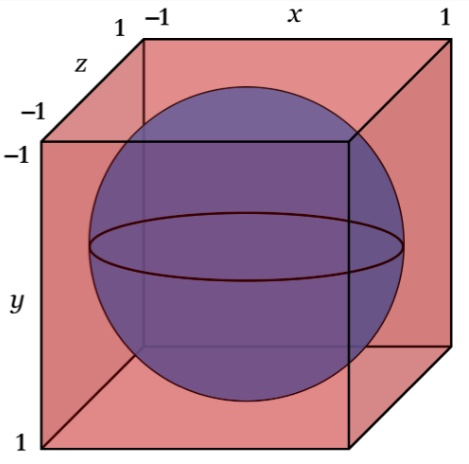
\includegraphics[width=.25\textwidth]{cube_sphere}
  \caption{To cover the volume of \(f(x)\) in higher dimensions we intuitively need a volume that grows exponentially with the dimension itself.}\label{fig:curse_dimensionality}
\end{figure}

MCMC methods are based on the iterative construction of a Markov chain whose stationary distribution is the objective distribution \(\pi(x)\). In this way, we can take the samples of a sufficiently advanced chain as approximate realizations of \(X\sim \pi(x)\). When it comes to building the chains, transition probabilities are assigned in such a way that regions with higher density with respect to \(\pi(x)\) are favored (by means of the known proportional function \(f(x)\)). The dimensionality issues are somewhat mitigated, and on top of that there are specific tuning techniques to tackle them. However, the samples obtained from this procedure are not independent, though they can be made so by \textit{thinning} the chain and considering only one every few samples.

Another advantage of these methods is that they recover the marginal distributions directly. Suppose that after a successful MCMC run we have \(M\) multivariate samples \(\{\theta^{(m)}=(\theta_1^{(m)},\dots, \theta_p^{(m)})\}\) of a joint \(p\)-dimensional distribution. The marginal distribution of each variable, which would be theoretically computed as
\[
\pi(\theta_i) = \int \pi(\theta)\,d\theta_1\,\cdots\,d\theta_{i-1}\,d\theta_{i+1}\,\cdots \,d\theta_p,
\]
can be approximated by just retaining the samples \(\{\theta_i^{(m)}\}\) corresponding to \(\theta_i\).

\subsection*{Metropolis-Hastings}

The Metropolis-Hastings algorithm \citep{metropolis1953equation} is arguably the best known algorithm in this context. As a matter of fact, it is actually more of a general framework from which many other methods are derived. In its original formulation, it relies on a symmetric \textit{proposal} distribution \(g(x'|x_t)\) that generates a proposal for the next state given the current one (e.g. a Gaussian distribution centered on \(x_t\)). Approximate samples from the intended distribution can then be generated through the following iterative acceptance-based procedure:
\begin{enumerate}[1.]
  \item Generate a proposal \(x' \sim g(x'|x_t)\).
  \item Accept the proposal with probability \(\alpha=\min\{1, f(x')/f(x_t)\}\). If accepted, set \(x_{t+1}=x'\); otherwise set \(x_{t+1}=x_t\).
\end{enumerate}

 \begin{figure}[ht!]
   \centering
   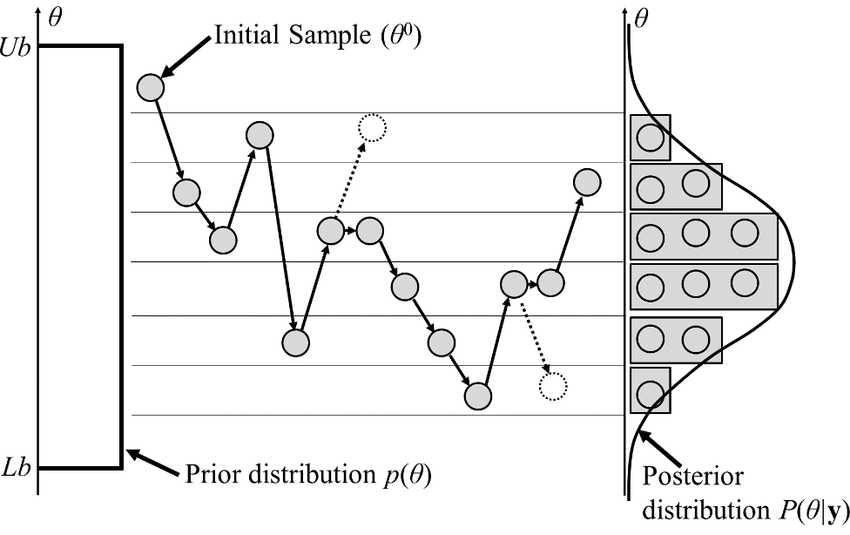
\includegraphics[width=.55\textwidth]{mh}
   \caption{Representation of the Metropolis-Hastings algorithm (taken from \citet{jaewook2015metamodel}). The discarded proposals are represented by dashed circles.}\label{fig:mh}
 \end{figure}

Figure~\ref{fig:mh} shows a schematic representation of the process. Note that \(f(x')/f(x_t)=\pi(x')/\pi(x_t)\) is a measure of how more likely is \(x'\) to be a sample from \(\pi\) than \(x_t\). This specific acceptance rate is also chosen so that the detailed balance equations of the chain are satisfied, i.e., \(\pi(x)P(x'|x)=\pi(x')P(x|x')\), where \(P(x|y)\) represents the transition probability from state \(x\) to state \(y\). These conditions essentially guarantee that \(\pi\) is the stationary distribution of the chain; see \citet{robert1999monte} for additional details. An immediate generalization consists on choosing a general (possibly non-symmetric) jump distribution \(g\), in which case the acceptance probability is rewritten as
\[
\alpha = \min\left\{1, \frac{f(x')g(x_t \mid x')}{f(x_t)g(x'\mid x_t)}\right\}.
\]

Although this algorithm performs well on a wide range of problems, it can be difficult to find a suitable jump distribution when the number of dimensions is high. If we know the conditional distribution of each variable on the rest of them, an alternative approach to sampling is \textit{Gibb's algorithm} \citep{geman1984stochastic}, which is a particular case of Metropolis-Hastings that considers separate samples for each dimension. Specifically, in each step we get unidimensional samples \textit{in turn} (e.g. via rejection sampling) of each variable conditional on the rest of them, using always the more up-to-date values available:

\[
\pi(x_l^{(i+1)} \mid x_{1}^{(i+1)}, \dots, x_{l-1}^{(i+1)}, x_{l+1}^{(i)}, \dots, x_L^{(i)}), \quad l=1,\dots,L.
\]

Lastly, there are several methods based on Metropolis-Hastings that are the subject of active research, both from a theoretical and computational standpoint. A good example are \textit{Hamiltonian Monte Carlo} methods \citep[e.g.][]{neal2011mcmc}, which are a family of algorithms that introduce gradient information to guide the proposals in the sample space. They are based on Hamiltonian dynamics, and in general they improve convergence speed due to a more intelligent choice of new points on the chain. With automatic differentiation being developed in the last few decades, these algorithms have become computationally feasible and have been widely adopted by the scientific community.

\subsection*{Affine-invariant ensemble sampler}

An interesting and often desirable property of sampling algorithms is that they be \textit{affine-invariant}, which means that they regard two distributions that differ in an affine transformation, say \(\pi(x)\) and \(\pi_{A, b}(Ax + b)\), as equally difficult to sample from. This is useful when one is working with very asymmetrical or skewed distributions, for an affine transformation can turn them into ones with simpler shapes.

Generally speaking, a MCMC algorithm can be described at time \(t+1\) as \(\Lambda(t+1)=R(\Lambda(t), \xi(t), \pi)\), where \(\Lambda(t)\) is the state of the chain at instant \(t\), \(\pi(x)\) is the objective distribution, and \(\xi(t)\) is a sequence of i.i.d. random variables that represent the random behavior of the chain. With this notation, the property of affine-invariant can be characterized as \citep{goodman2010ensemble}:
 \[
 R(A\lambda+b, \xi(t), \pi_{A,b}) = AR(\lambda, \xi(t), \pi) + b,
 \]
 for all \(A,b\) and \(\lambda\), and for almost all \(\xi(t)\). This means that if we fix a random generator and run the algorithm twice, one time using \(\pi\) and starting in \(\Lambda(0)\) and a second time using \(\pi_{A,b}\) with initial point \(\Gamma(0)=A\Lambda(0)+b\), then \(\Gamma(t)=A\Lambda(t)+b\) for all \(t\). In \citet{goodman2010ensemble} the authors consider an ensemble of samplers with the affine invariance property. Specifically, they work with a set \(\Lambda=(\Lambda_1, \dots, \Lambda_L)\) of \textit{walkers}, where \(\Lambda_l(t)\) represents an individual chain at time \(t\). At each iteration, an affine-invariant transformation is used to find the next point, which is constructed using the current values of the rest of the walkers (similar to Gibb's algorithm), namely the \textit{complementary ensemble}
 \[
  \Lambda_{-l}(t) = \{\Lambda_1(t+1), \dots, \Lambda_{l-1}(t+1), \Lambda_{l+1}(t), \dots, \Lambda_L(t)\}, \quad l=1,\dots, L.
  \]

To maintain the affine invariance and the joint distribution of the ensemble, the walkers are advanced one by one following a Metropolis-Hastings acceptance scheme. There are mainly two types of moves.

  \paragraph{Stretch move.} For each walker \(1\leq l \leq L\) another walker \(\Lambda_j \in \Lambda_{-l}(t)\) is chosen at random, and the proposal is constructed as
  \[
    \Lambda_l(t) \to \Gamma = \Lambda_j + Z(\Lambda_l(t) - \Lambda_j),
  \]
  where \(Z \stackrel{i.i.d.}{\sim} g(z)\) satisfying the symmetry condition \(g(z^{-1})=zg(z)\). In particular, the suggested density is
  \[
  g_a(z) \propto \begin{cases}
    \frac{1}{\sqrt{z}}, & \text{if } z \in [a^{-1}, a],\\
    0, & \text{otherwise.}
\end{cases}, \quad a > 1.
  \]
Supposing \(\R^p\) is the sample space, the corresponding acceptance probability (chosen so that the detailed balance equations are satisfied) is:
  \[
    \alpha = \min\left\{1, \ Z^{p-1}\frac{\pi(\Gamma)}{\pi(\Lambda_l(t))}\right\}.
  \]

  \paragraph{Walk move.} For each walker \(1\leq l \leq L\) a random subset \(S_l \subseteq \Lambda_{-l}(t)\) with \(|S_l| \geq 2\) is chosen, and the proposed move is
\[
\Lambda_l(t) \to \Gamma = \Lambda_l(t) + W,
\]
where \(W\) is a normal distribution with mean \(0\) and the same covariance as the sample covariance of all walkers in \(S_l\). The acceptance probability in this case is just the Metropolis ratio, i.e., \(\alpha=\min\{1, \pi(\Gamma)/\pi(\Lambda_l(t))\}\).\\

From a computational perspective, the Python library \textit{emcee}\footnote{\url{https://emcee.readthedocs.io/en/stable/}} \citep{foreman2013emcee} provides a parallel implementation of this algorithm. The idea is to divide the ensemble \(\Lambda\) into two equally-sized subsets \(\Lambda^{(0)}\) and \(\Lambda^{(1)}\), and then proceed on each iteration in the following alternate fashion:

\begin{enumerate}[1.]
  \item Update \textit{all} walkers in \(\Lambda^{(0)}\) through one of the available moves explained above, using \(\Lambda^{(1)}\) as the complementary ensemble.
  \item Use the new values in \(\Lambda^{(0)}\) to update \(\Lambda^{(1)}\).
\end{enumerate}

In this way the detailed balance equations are still satisfied, and each of the steps can benefit from the computing power of an arbitrary number of processors (up to \(L/2\)).

%%%%%%%%%%%%%%%%%%%%%%%%%%%%%%%%%%%%%%%%%%%%%%%%%%%%%%%%%%%%%%%%%%%%%%%%
% Copyright (c) 2022 Antonio Coín
%
% This work is licensed under a
% Creative Commons Attribution-ShareAlike 4.0 International License.
%
% You should have received a copy of the license along with this
% work. If not, see <http://creativecommons.org/licenses/by-sa/4.0/>.
%%%%%%%%%%%%%%%%%%%%%%%%%%%%%%%%%%%%%%%%%%%%%%%%%%%%%%%%%%%%%%%%%%%%%%%%

\let\epsilon\varepsilon
\setlength{\footskip}{50.75pt}

%%%%%%%%%%%%%%%%%%%%%%%%%%%%%%%%%%%%%%%%%%%%%%%%%%%%%%%%%%%%%%%%%%%%%%%%
\chapter{Bayesian methodology for RKHS-based functional regression models}\label{ch:bayesian}
%%%%%%%%%%%%%%%%%%%%%%%%%%%%%%%%%%%%%%%%%%%%%%%%%%%%%%%%%%%%%%%%%%%%%%%%

In this chapter we present the precise functional models and Bayesian methodologies explored in this work. The RKHS-based functional models under consideration \citep[see][]{berrendero2018functional, berrendero2019rkhs} are those obtained by substituting the functional parameter \(\beta\in L^2[0,1]\) for \(\alpha \in \Hcal(K)\), replacing also the scalar product \(\dotprod{X}{\beta}\) for \(\dotprod{X}{\alpha}_K\) in the \(L^2\)-models~\eqref{eq:l2-linear-model} and~\eqref{eq:l2-logistic-model}. However, to further simplify things we will follow a parametric approach and suppose that \(\alpha\) is in fact a member of the dense subspace \(\Hcal_0(K)\) defined in~\eqref{eq:h0}, i.e.:
\begin{equation}\label{eq:alpha_h0}
\alpha(\cdot) = \sum_{j=1}^p \beta_j K(t_j, \cdot), \text{ for some } p \in \N, \ \beta_j \in \R \text{ and } t_j \in [0,1].
\end{equation}
Moreover, as we said before, with a slight abuse of notation we will understand the expression \(\dotprod{x}{\alpha}_K\) as \(\Psi_x(\alpha)\), where \(x=X(\omega)\) and \(\Psi_x\) is Loève's isometry. Hence, taking into account that \(\Psi_X(K(t, \cdot)) = X(t)\) by definition (see~\eqref{eq:loeves-isometry}), when \(\alpha\) is as in~\eqref{eq:alpha_h0} we can write \(\dotprod{x}{\alpha}_K \equiv \sum_{j=1}^p \beta_j x(t_j)\).

In this way we get a simpler, finite-dimensional approximation of the functional RKHS model, which we argue reduces the overall complexity of the model while still capturing most of the relevant information. When it comes to parameter estimation, a direct optimization of some loss function would probably require a tailored algorithm that took into account the continuous nature of the times \(t_j\). Indeed, such an idea is explored in \citet{berrendero2018functional} for the logistic regression case, where the authors propose a ``greedy max-max'' method reminiscent of the EM algorithm that alternates between estimating the coefficients and the time instants through a maximum likelihood approach.

At this point we propose to follow a Bayesian approach to estimate the parameters of the model, which we believe is in line with the idea of simplicity we pursue, and also introduces an additional layer of flexibility into the model. In this way, we can include problem-specific information through the use of prior distributions, and on top of that, this method works almost unaltered for both linear and logistic regression models. The general idea will be to impose a prior distribution on the functional parameter to eventually derive a posterior distribution after incorporating the available sample information.

In view of~\eqref{eq:alpha_h0}, to set a prior distribution on the unknown function \(\alpha\) (that is, a prior distribution on the functional space \(\Hcal_0(K)\)) it suffices to first consider a discrete distribution on \(p\), and then impose \(p\)-dimensional continuous prior distributions on the coefficients \(\beta_j\) and the times \(t_j\) given \(p\). Thanks to this parametric approach, the challenging task of setting a prior distribution on a space of functions is considerably simplified, while simultaneously not constraining the model to any specific distribution (in contrast to, for instance, Gaussian process regression methods). Moreover, note that starting from a probability distribution \(\P_0\) on \(\Hcal_0(K)\) we can obtain a probability distribution \(\P\) on \(\Hcal(K)\) merely by defining \(\P(B) = \P_0(B\cap \Hcal_0(K))\) for all Borel sets \(B\). Consequently, our simplifying assumption on \(\alpha\) is not actually very restrictive, since any prior distribution on \(\Hcal_0(K)\) can be directly extended to a prior distribution on \(\Hcal(K)\).

However, after some initial experimentation we found that, for practical and computational reasons, the value of \(p\) (the dimensionality of the model) is best fixed beforehand in a suitable way; see Chapter~\ref{ch:model-choice} for details. Thus, we will regard only the \(\beta_j\) and \(t_j\) as free parameters, and search for our functional parameter in the space
\begin{equation}\label{eq:h0p}
\Hcal_{0,p}(K)=\left\{ \sum_{j=1}^p \beta_j K(t_j, \cdot): \ \beta_j \in \R, \ t_j \in [0, 1]\right\}.
\end{equation}
Even though we actually work on \(\Hcal_{0,p}(K)\), the discrete parameter \(p\) can still be selected in several meaningful ways that make use of the available data, and the set of feasible values is not very large in practice. Moreover, we could think of this approach as imposing a degenerate prior distribution on \(p\), so it is in a way a particular case of the more general model discussed above.

In any case, after selecting a suitable prior distribution \(\pi(\theta)\) for the finite-dimensional parameter vector \(\theta\) (which will be specified shortly), we can resort to Bayes' theorem to perform the inference step, which in the case of i.i.d. samples amounts to
\begin{equation}\label{eq:bayes-theorem}
  \pi(\theta \mid \D_n) \propto \left( \prod_{i=1}^n \pi(Y_i\mid X_i, \theta) \right)\pi(\theta).
\end{equation}
In Sections~\ref{sec:rkhs-linear-model} and~\ref{sec:rkhs-logistic-model} we proceed to specify the parameter spaces, prior distributions and concrete models for \(\pi(Y | X,\theta)\) considered in the case of functional linear regression and functional logistic regression, respectively. Even though in~\eqref{eq:bayes-theorem} we have omitted the possibly intractable integral related to the normalizing constant, sampling from the (approximate) posterior distribution can still be accomplished via MCMC methods (see Chapter~\ref{ch:model-choice} for implementation details).

\section{Functional linear regression}\label{sec:rkhs-linear-model}

In the case of functional linear regression, the simplified RKHS model considered is
\begin{equation}\label{eq:rkhs-model-linear}
  Y = \alpha_0 + \dotprod{X}{\alpha}_K + \epsilon = \alpha_0 + \sum_{j=1}^p \beta_j X(t_j) + \epsilon,
\end{equation}
where \(\alpha(\cdot) = \sum_{j=1}^p \beta_j K(t_j, \cdot) \in \Hcal_{0,p}(K)\), \(\alpha_0\in\R\), and \(\epsilon \sim \mathcal N(0, \sigma^2)\) is an error term independent from \(X\). This model is essentially a finite-dimensional approximation from a functional perspective to the more general RKHS model that assumes \(\alpha \in \Hcal(K)\), proposed in~\citet{berrendero2019rkhs}.

When \(p\) is fixed, the parameter space becomes \(\Theta_p = \R^p \times [0, 1]^p \times \R \times \R^+\), and in the sequel a generic element of this \((2p+2)\)-dimensional space will be denoted by \(\theta = (\beta_1,\dots, \beta_p, t_1,\dots, t_p, \alpha_0, \sigma^2) \equiv (b, \tau, \alpha_0, \sigma^2)\). Before proceeding further, observe that we can rewrite model~\eqref{eq:rkhs-model-linear} in a more explicit and practical fashion in terms of the available sample information in \(\D_n\). Indeed, for \(\theta \in \Theta_p\) the reinterpreted model assumes the form
\begin{equation}\label{eq:rkhs-model-linear-2}
  Y_i \mid X_i, \theta \ \stackrel{\text{i.i.d.}}{\sim} \mathcal N\left(\alpha_0 + \sum_{j=1}^p \beta_j X_i(t_j), \ \sigma^2\right), \quad i =1,\dots, n.
\end{equation}

It is worth mentioning that the model remains linear in the sense that it fundamentally involves a random variable \(\dotprod{X}{\alpha}_K = \Psi_X(\alpha)\) belonging to the linear span of the process \(X\) in \(L^2(\Omega)\). Also, note that given the time instants \(t_j\), the model becomes a multiple linear model with the \(X(t_j)\) as scalar covariates. As a matter of fact, this model is particularly suited as a basis for variable selection methods, and furthermore the general RKHS model entails the classical \(L^2\)-model~\eqref{eq:l2-linear-model} under certain conditions \citep[see][Sec.~3]{berrendero2020general}. In addition, this model could be easily extended to the case of several covariates via an expression of type \(Y=\alpha_0 + \dotprod{X^1}{\alpha_1}_K + \cdots + \dotprod{X^q}{\alpha_q}_K + \epsilon\). In that case, as argued in \citet{grollemund2019bayesian} for a similar situation, if we were to set a prior distribution on all the parameters involved, we could recover the full posterior by looking alternately at the posterior distribution of each covariate conditional on the rest of them.

\enlargethispage{1\baselineskip}

\subsection*{The Bayesian approach: prior and posterior}

The prior distribution suggested for the parameter vector \(\theta \in \Theta_p\) is given by
\begin{align}\label{eq:prior-linear}
  \begin{split}
  \pi(\alpha_0, \sigma^2)              & \propto 1/\sigma^2,                                                     \\
  \tau                     & \sim \U([0, 1]^p),                                              \\
  b\mid \tau, \sigma^2 & \sim \mathcal N_p(b_0, g\sigma^2{\underbrace{\left(\X_\tau' \X_\tau + \eta I\right)}_{G_\tau}}^{-1}),
\end{split}
\end{align}
where \(I\) is the identity matrix, \(\X_\tau\) is the data matrix \((X_i(t_j))_{i,j}\), and \(b_0\in \R^p, \ g \in \R\) and \(\eta \in \R^+\) are hyperparameters of the model. On the one hand, note the use of a joint prior distribution on \(\alpha_0\) and \(\sigma^2\), which is a widely used non-informative prior known in the standard linear regression setting as Jeffrey's prior \citep{jeffreys1946invariant}. In any event, the estimation of \(\alpha_0=\E[Y]\) is straightforward, so it could have been left out of the model altogether. On the other hand, the prior on \(b\) is a slight modification of the well-known Zellner's g-prior \citep{zellner1986assessing}, in which a regularizing term is added to avoid ill-conditioning problems in the Gram matrix, obtaining a ridge-like Zellner prior controlled by the tuning parameter \(\eta\) \citep{baragatti2012study}. All in all, with a slight abuse of notation the proposed prior distribution becomes \(\pi(\theta) = \pi(b| \tau, \sigma^2)\pi(\tau)\pi(\alpha_0, \sigma^2)\).

As for the posterior distribution, we only compute a function proportional to its log-density, since that is all that is needed for a MCMC algorithm to work. A standard algebraic manipulation in~\eqref{eq:bayes-theorem} yields the following result.

\begin{proposition}
Under the linear model~\eqref{eq:rkhs-model-linear-2}, the prior distribution implied in~\eqref{eq:prior-linear} produces the log-posterior distribution
\begin{align*}
\log \pi(\theta \mid \D_n) \propto {} & \frac{1}{2\sigma^2}\left(\|\symbf Y- \alpha_0\symbf{1} - \X_\tau b\|^2 + \frac{1}{g}(b - b_0)'G_\tau(b - b_0) \right)\\
& + (p+n+2)\log\sigma - \frac{1}{2}\log |G_\tau|,
\end{align*}
where \(\symbf Y=(Y_1,\dots,Y_n)'\) and \(\symbf{1}\) is an \(n\)-dimensional vector of ones.
\end{proposition}

\subsection*{Making predictions}

In order to generate predictions, let us recall that when performing the empirical posterior approximation, on each of the \(M\) steps of the iterative MCMC algorithm we get an approximate sample \(\theta^{(m)*}=(b^{(m)*}, \tau^{(m)*}, \alpha_0^{(m)*}, (\sigma^2)^{(m)*})\) of the posterior distribution \(\pi(\theta| \D_n)\). Assuming now a previously unseen test set \(\D'_{n'}\) in the same conditions as \(\D_n\), we propose to construct three different kinds of predictors based on the MCMC samples, each of them following a different strategy.

  \paragraph{Summarize-then-predict.} If we consider a point-estimate statistic \(T\) that acts as a summary of the marginal posterior distributions, we can get the corresponding estimates \(\hat{\theta}=(\hat b, \hat \tau, \hat{\alpha}_0, \hat{\sigma}^2) = T\{\theta^{(m)*}\} \equiv (T\{b^{(m)*}\}, T\{\tau^{(m)*}\}, T\{\alpha_0^{(m)*}\}, T\{(\sigma^2)^{(m)*}\})\), and then we can predict the responses in the usual way following model~\eqref{eq:rkhs-model-linear}, i.e.:
  \begin{equation}\label{eq:summarize-predict-linear}
    \hat Y_i = \hat{\alpha}_0 + \sum_{j=1}^p \hat{\beta}_j X_i(\hat{t}_j), \quad i=1,\dots, n'.
  \end{equation}
  Note that in this case the variance \(\sigma^2\) is treated as a nuisance parameter. Although it contributes to measure the uncertainty in the approximations, its estimates are discarded in the final prediction.

  \paragraph{Predict-then-summarize.} Alternatively, we can  look at the approximate posterior distribution as a whole, and compute the predictive distribution of the simulated responses at each step of the chain following model~\eqref{eq:rkhs-model-linear-2}:
  \begin{equation}\label{eq:sampled-response-vector}
  \symbf Y^{(m)*} := \left\{Y_i^{(m)*} \equiv Y_i \mid X_i, \theta^{(m)*}:\ i=1,\dots,n'\right\}, \quad m=1,\dots,M.
  \end{equation}
  Then, we can take the mean of all such simulated responses as a proxy for each response variable, that is,
  \[
  \hat Y_i = \frac{1}{M}\sum_{m=1}^M Y_i^{(m)*}, \quad i=1,\dots,n'.
  \]
  This method differs from the previous one in that it takes into account the full approximate posterior distribution instead of summarizing it directly.

  \paragraph{Variable selection.} Lastly, we can focus only on the marginal posterior distribution of \(\tau|\D_n\) and select \(p\) time instants using a point-estimate statistic \(T\) as in our first strategy, but discarding the rest of the parameters. Specifically, we can consider the times \(\hat t_j = T\{t_j^{(m)*}\}\) and reduce the original data set to just the \(n\times p\) real matrix given by \(\{X_i(\hat t_j): i=1, \dots,n, \ j=1,\dots,p\}\). After this variable selection has been carried out, we can tackle the problem using a finite-dimensional linear regression model and apply any of the well-known prediction algorithms suited for this situation.\\

Note that these predictors can be obtained all at once after only one round of training (that is, an individual MCMC run to approximate the posterior distribution). As a consequence, what we have in practice is a single algorithm that can produce multiple predictors at the same computational cost, so that any of them can be chosen (or even switched back and forth) depending on the particularities of the problem at hand. Moreover, one could even contemplate an \textit{ensemble model} in which some kind of aggregation of several of the available prediction methods is performed to produce a final result.

Besides, observe that the choice of a specific point estimator to summarize the posterior distribution results in a veiled assumption of an underlying loss function between the estimated and real parameters. In general, the mean is more sensitive to outliers and the median is more robust, but the latter assumes an \(l^1\)-type loss function while the former implicitly optimizes an \(l^2\) loss. On the other hand, the mode is also a good candidate because it represents the point of highest probability density, following a \textit{maximum a posteriori} (MAP) approach. At any rate, these decisions are strongly dependent on several factors such as the skewness or the number of modes in the resulting posterior distribution, and thus should be made on a case-by-case basis.

\newpage

\section{Functional logistic regression}\label{sec:rkhs-logistic-model}

In the case of functional logistic regression, we regard the response variable \(Y\in\{0, 1\}\) as a Bernoulli random variable given \(X=x \in L^2[0, 1]\), and as usual suppose that \(\log\left(p(x)/(1-p(x))\right)\) is linear in \(x\), where \(p(x)=\P(Y=1| X=x)\). Then, following the approach  suggested by \citet{berrendero2018functional}, a RKHS model might be given, in terms of the correspondence \(\dotprod{X}{\alpha}_K = \Psi_X(\alpha)\), by the equation
\begin{equation}\label{eq:rkhs-model-logistic}
  \P(Y=1 \mid X) = \frac{1}{1 + \exp\{-\alpha_0 - \dotprod{X}{\alpha}_K\}}, \quad \alpha_0 \in \R, \ \alpha \in \Hcal_{0,p}(K).
\end{equation}

Indeed, note that this can be seen as a finite-dimensional approximation (but, still, with a functional interpretation) to the general RKHS functional logistic model proposed by these authors, which can be obtained by replacing \(\Hcal_{0,p}(K)\) with the whole RKHS space \(\Hcal(K)\). Now, if we aim at a classification problem, our strategy will be similar to that followed in the functional linear model: after incorporating the sample information, we can rewrite~\eqref{eq:rkhs-model-logistic} as
\begin{equation}\label{eq:rkhs-model-logistic-2}
Y_i \mid X_i,\theta \ \stackrel{\text{i.i.d.}}{\sim} \operatorname{Bernoulli}(p_i), \quad i=1,\dots, n,
\end{equation}
with
\begin{equation}\label{eq:rkhs-model-logistic-2-parameter}
  p_i = \P(Y_i=1 \mid X_i,\theta) = \frac{1}{\displaystyle 1 + \exp\left\{-\alpha_0 - \sum_{j=1}^p \beta_j X_i(t_j)\right\}}, \quad i=1,\dots, n,
\end{equation}
where in turn \(\alpha_0, \beta_j\in\R\) and \(t_j\in[0, 1]\).

In much the same way as the linear regression model described above, this RKHS-based logistic regression model offers some advantages over the \(L^2\)-model~\eqref{eq:l2-logistic-model}. First and foremost, it has a more straightforward interpretation and allows for a workable Bayesian approach, as we will demonstrate below. Secondly, it can be shown that under mild conditions the general RKHS functional logistic model holds whenever the conditional distributions \(X | Y=0\) and \(X|Y=1\) are homoscedastic Gaussian processes, and in some cases it also entails the \(L^2\)-model \citep[see Theorem 1 in][]{berrendero2018functional}; this provides a sound theoretical motivation for the reduced model. Furthermore, a maximum likelihood approach for parameter estimation (although not considered here) is possible as well. Indeed, the use of a finite-dimensional approximation  mitigates the problem of non-existence of the MLE in the functional case. However, let us recall that even in finite-dimensional settings there are cases of quasi-complete separation in which the MLE does not exist \citep{albert1984existence}, though this issue can be circumvented using, for example, Firth's corrected estimator \citep{firth1993bias}.

\subsection*{The Bayesian approach: prior and posterior}

As far as prior distributions go, we propose to use the same ones as we did in~\eqref{eq:prior-linear} for the linear regression model. However, in this case the nuisance parameter \(\sigma^2\) only appears as part of the hierarchical prior distribution, and not in the final model. The posterior distribution is again derived after a routine calculation.

\begin{proposition}
Under the logistic model~\eqref{eq:rkhs-model-logistic-2}, the prior distribution implied in~\eqref{eq:prior-linear} produces the log-posterior distribution
\begin{align*}
  \log \pi(\theta \mid \D_n) \propto {} & \sum_{i=1}^n \left[ \left(\alpha_0 + \dotprod{X_i}{\alpha}_K\right)Y_i - \log\left(1 + \exp\left\{\alpha_0 + \dotprod{X_i}{\alpha}_K\right\}\right)\right]\\
  \quad &+ \frac{1}{2}\log |G_\tau| - (p+2)\log \sigma -\frac{1}{2g\sigma^2} (b - b_0)'G_\tau(b - b_0).
\end{align*}
Remember that \(\dotprod{X_i}{\alpha}_K = \sum_{j=1}^p \beta_j X_i(t_j)\).
\end{proposition}

\subsection*{Making predictions}

Bear in mind that in this case we are essentially approximating the probabilities \(p_i\) in~\eqref{eq:rkhs-model-logistic-2-parameter}, so before producing a response we need to transform the predicted values to a binary output in \(\{0, 1\}\). According to the usual criterion of minimizing the misclassification probability, it is known that the Bayes optimal rule is recovered by predicting \(\hat Y=1\) whenever \(\P(Y=1|X) \geq 1/2\). Nevertheless, for a more general cost function one could consider other criteria that would lead to evaluating whether \(\P(Y=1|X) \geq \gamma\) for some threshold \(\gamma\in[0, 1]\).

With this last strategy in mind, the summarize-then-predict approach on the approximate posterior distribution is analogous to the linear regression case:
\begin{equation}\label{eq:summarize-predict-logistic}
\hat Y_i = \I \left( \left[\displaystyle 1 + \exp\left\{-\hat\alpha_0 - \sum_{j=1}^p \hat\beta_j X_i(\hat t_j)\right\}\right]^{-1} \geq \gamma \right), \quad i=1,\dots,n',
\end{equation}
where \(\I\) is the indicator function (\(\I(P)\) is \(1\) if \(P\) is true and \(0\) otherwise). The hat estimates are obtained once again through a summary statistic \(T\) of the corresponding marginal posterior distributions. On the other hand, the prediction method that takes into account the entire posterior approximation (i.e. the predict-then-summarize approach) is somewhat different now, since there is the question of which response (the Bernoulli variables in~\eqref{eq:rkhs-model-logistic-2} or the raw probabilities in~\eqref{eq:rkhs-model-logistic-2-parameter}) to consider when averaging the posterior samples. Hence, there are primarily two possible outcomes.

  \paragraph{Average sampled probability.} If we choose to average the approximate probabilities \(p_i^{(m)*} = \P(Y_i =1 | X_i,\theta^{(m)*})\) computed following~\eqref{eq:rkhs-model-logistic-2-parameter}, the resulting predictor is
  \[
    \hat Y_i = \I\left(\frac{1}{M} \sum_{m=1}^M p_i^{(m)*} \geq \gamma\right), \quad i=1,\dots,n'.
  \]
  \paragraph{Average sampled response.} Deciding to average the approximate binary responses \(Y_i^{(m)*}\) instead (see~\eqref{eq:sampled-response-vector}) leads to computing the predictions as
  \[
    \hat Y_i = \I\left(\frac{1}{M} \sum_{m=1}^M Y_i^{(m)*} \geq \gamma\right), \quad i=1,\dots,n'.
  \]
  In this case, each \(Y_i^{(m)*}\) is a random variable that follows a Bernoulli distribution with parameter \(p_i^{(m)*}\), for \(m=1,\dots,M\). Note that when \(\gamma=1/2\) this is equivalent to predicting \(\hat Y_i\) according to the majority vote of all the \(Y_i^{(m)*}\).\\

Lastly, the variable selection method is essentially the same as in the case of functional linear regression: we select \(p\) time instants from each trajectory based on a summary of the posterior distribution \(\tau | \D_n\), and then feed the reduced data set to a finite-dimensional binary classification procedure.

%%%%%%%%%%%%%%%%%%%%%%%%%%%%%%%%%%%%%%%%%%%%%%%%%%%%%%%%%%%%%%%%%%%%%%%%
% Copyright (c) 2022 Antonio Coín
%
% This work is licensed under a
% Creative Commons Attribution-ShareAlike 4.0 International License.
%
% You should have received a copy of the license along with this
% work. If not, see <http://creativecommons.org/licenses/by-sa/4.0/>.
%%%%%%%%%%%%%%%%%%%%%%%%%%%%%%%%%%%%%%%%%%%%%%%%%%%%%%%%%%%%%%%%%%%%%%%%

%%%%%%%%%%%%%%%%%%%%%%%%%%%%%%%%%%%%%%%%%%%%%%%%%%%%%%%%%%%%%%%%%%%%%%%%
\chapter{Model choice, implementation and validation}\label{ch:model-choice}
%%%%%%%%%%%%%%%%%%%%%%%%%%%%%%%%%%%%%%%%%%%%%%%%%%%%%%%%%%%%%%%%%%%%%%%%

In this chapter we gather together several remarks on the main choices made during the design and implementation of our model, as well as some examples of validation strategies that attempt to measure the goodness-of-fit of the model given the observed data.

\section{Model specification}

First we describe some problems and modeling decisions that we had to deal with throughout the development of the model.

\subsection*{Label switching}

A well-known issue found in mixture-like models like the ones we propose is \textit{label switching}, which in short refers to the non-identifiability of the components of the model caused by their interchangeability. In our case, this happens because the likelihood is symmetric with respect to the ordering of the parameters \(b\) and \(\tau\), i.e., \(\pi(Y|X,\theta)=\pi(Y|X, \nu(\theta))\) for any permutation \(\nu\) that rearranges the indices \(j=1,\dots, p\). Thus, since the components are arbitrarily ordered, they may be inadvertently exchanged from one iteration to the next in any MCMC algorithm. This can cause nonsensical answers when summarizing the marginal posterior distributions to perform inference, as different labelings might be mixed on each component \citep{stephens2000dealing}.

However, this phenomenon is perhaps surprisingly a condition for the convergence of the MCMC method: as pointed out by many authors \citep[e.g.][]{celeux2000computational}, a lack of switching would indicate that not all modes of the posterior distribution were being explored by the sampler. For this reason, many ad-hoc solutions revolve around post-processing and relabeling the samples to eliminate the switching effect, but they generally do not prevent it from happening in the first place.

The most straightforward solutions consist on imposing an artificial identifiability constraint on the parameters to break the symmetry of their posterior distributions; see \citet{jasra2005markov} and references therein. A common approach that seems to work well is to simply impose an ordering in the parameters in question, which in our case would mean requiring for example that \(\beta_i < \beta_j\) for \(i < j\), or the analogous with \(\tau\). We have implemented a variation of this method described in \citet{simola2021approximate}, which works by post-processing the samples and relabeling the components to satisfy the order constraint mentioned above, choosing either \(b\) or \(\tau\) depending on which set of ordered parameters would produce the largest separation between any two of them (suitably averaged across all iterations of the chains).

This is an area of ongoing research, and thus there are other, more complex relabeling strategies, both deterministic and probabilistic. A summary of several such methods can be found for example in \citet{rodriguez2014label} and \citet{papastamoulis2015label}. In particular, we tested the pivot method proposed by \citet{marin2005bayesian}, in which all samples are aligned to minimize their distance to a reference element (the ``pivot''), which is chosen as the sample that maximizes the posterior density. However, the process of finding the appropriate permutation in each case was time-consuming, and the results were similar, if not worse, than the ones obtained with the simpler order constraints, so the latter were chosen as the default relabeling method of our algorithm (though the pivot method can still be enabled through a dedicated argument in the sampling procedure).

\subsection*{The choice of \(p\)}

One of the key decisions in our Bayesian modeling scheme was whether to consider the number of components \(p\) as a member of the parameter space and integrate it into the model. While theoretically we could impose a prior distribution on \(p\) as well (e.g. a categorical distribution with a fixed maximum value), we found that it would have some unwanted practical implications. For instance, it would make the implementation more complex, since the dimensionality of the parameters \(b\) and \(\tau\) would need to be fixed at a certain maximum value beforehand, but the working value of \(p\) within the MCMC algorithm would vary from one iteration to the next. In this case we would have no immediate way of tracking down which set of parameters is ``active'' at any given time. A simple approach would be to always consider the first \(p\) parameters and ignore the rest, and we did indeed try this technique, but it gave rise to new difficulties and the results obtained were not good. In fact, the label switching issue is accentuated when \(p\) is allowed to vary \citep[c.f.][Sec.~2.3]{grollemund2019bayesian}, and on top of that, the interpretation of, say, the first coefficient \(\beta_1\) in a model with \(3\) components is different than the interpretation of the same coefficient in a model with only \(2\) components.

This inconsistency in the interpretation of the components when the dimensionality of the model increases or decreases can be mitigated using a particular type of MCMC method known as reversible-jump MCMC \citep{green1995reversible}. Theoretically, these algorithms are specifically designed to approximate the posterior distribution in mixture-like models when the number of components is unknown, allowing the underlying dimensionality to change between iterations. However, since they are not yet widely adopted in practice and a reference implementation is not available, we decided against using them in our applications.

Another possibility would be to adapt a purely Bayesian model selection technique to our framework \citep[see][]{piironen2017comparison, gelman2013bayesian}, or even derive some model aggregation methods to combine the posterior distributions obtained for different-sized models. These methods are usually based in computing a quantity known as the \textit{Bayes factor}, which in turn needs the normalizing integral constant we have been trying to avoid all along. In the end, for the sake of simplicity we decided to let \(p\) be an hyperparameter, so that we could use any model selection criteria (e.g. BIC, DIC, cross-validation, \ldots) to select its optimal value. As we will see shortly in Chapter~\ref{ch:experiments}, the experiments carried out indicate that even low values of \(p\) provide sufficient flexibility in most scenarios.

\subsection*{Other hyperparameters}

As for the default values of the rest of hyperparameters in the prior distributions in~\eqref{eq:prior-linear}, several comments are in order:
\begin{itemize}
  \item For the expected value \(b_0\) we propose to use the MLE of \(b\). Although the likelihood function is rather involved, an approximation of the optimal value is enough for our purposes. Our numerical studies suggest that the results are much better with this choice than, say, with a random or null vector.
  \item We found that the parameter \(g\) does not have as much influence on the final result, and the experimentation indicates that \(g=5\) is a good value.
  \item Lastly, we observed that the choice of \(\eta\) can have a considerable impact on the final estimator. That is why, in an effort to normalize its scale, we consider a compound parameter \(\eta = \tilde \eta \lambda_{\max}(\mathcal X_\tau'\mathcal X_\tau)\), where \(\lambda_{\max}(\mathcal X_\tau'\mathcal X_\tau)\) is the largest eigenvalue of the matrix \(\mathcal X_\tau'\mathcal X_\tau\), and \(\tilde\eta > 0\) is the actual tuning parameter (which can be selected for instance by cross-validation strategies). This standardization technique has been used previously in the literature; see for example \citet{grollemund2019bayesian}.
\end{itemize}

\section{MCMC implementation}

The MCMC method chosen for approximating the posterior distribution in our models is the affine-invariant ensemble sampler described in Section~\ref{sec:mcmc}. As mentioned there, we utilize the computational implementation in the Python library \textit{emcee}, which is both reliable and easy to use; it aims to be a general-purpose package that performs well in a wide class of problems. One advantage of this method, apart from the property of affine-invariance, is that it only requires us to specify a few hyperparameters, irrespective of the underlying dimension. This contrasts to, say, the \(\mathcal O(N^2)\) degrees of freedom corresponding to the covariance matrix of an \(N\)-dimensional jump distribution in Metropolis-Hastings.
Furthermore, following \citet{goodman2010ensemble} we can use the \textit{integrated autocorrelation time} to compute an estimate of the effective sample size (i.e. the number of independent samples) after the sampling is done.

After selecting the number of iterations and the number of chains we want, we need to specify the initial points for each of them. As pointed out in \citet{foreman2013emcee}, a good initial choice is a Gaussian ball around a point in \(\Theta_p\) that is expected to have a high probability with respect to the objective distribution. In our implementation we adopt this method, choosing an approximation of the MLE of \(\theta\) as the central point in each case. To perform this approximation we employ the optimization suite of the Python library \textit{scipy}\footnote{\url{https://docs.scipy.org/doc/scipy/}}, and in particular we use the Basin-hopping algorithm \citep{wales1997global}. This is a two-phase stochastic method that combines global steps with local optimization, in the hope of avoiding getting stuck too quickly in local maxima. To reduce the effects of randomness, we run the algorithm a few times and retain the point with the highest likelihood, and to avoid biasing the sampler too much towards the specific point selected, we let a fraction of the initial points be random (within reasonable bounds). This approximation is also used to specify the hyperparameter \(b_0\).

Other less relevant hyperparameters include the burn-in period for the chains, which is the number of initial samples discarded, or the amount of thinning performed, which is the number of consecutive samples discarded to reduce the correlation among them. Another computational decision we made is working with \(\log \sigma\) instead of \(\sigma^2\), so that the domain of this parameter is an unconstrained space, which apparently helps increase the efficiency of the method.

Finally, it is worth mentioning that we experimented with another MCMC framework called \textit{pymc}\footnote{\url{https://docs.pymc.io}}. This is a well-established project aimed at developing a probabilistic programming language for Bayesian modeling with emphasis on MCMC methods \citep{salvatier2016probabilistic}. This package is more complex to use and has a steeper learning curve, but at the same time offers a richer experience and a wide variety of samplers. Apart from standard Metropolis-Hastings techniques, the main algorithm in this library is the \textit{No U-Turn Sampler} (NUTS), a Hamiltonian Monte Carlo method proposed in \citet{hoffman2014no} that performs an automatic adjustment of hyperparameters. However, while the results obtained were similar to that of \textit{emcee}, the execution time of the NUTS sampler was considerably higher (most likely due to parametrization issues with the model). Nevertheless, we decided to include this package as part of the developed code for future use (the Metropolis-Hastings sampler is fully functional and shows comparable performance to \textit{emcee}), although we do not report the corresponding experimental results.

\section{Validation techniques}

To conclude, it is worth mentioning that the Bayesian aspects of our model allow us to perform some model validation checks straight away. For example, we can derive credible intervals for each of the parameters (see Figure~\ref{fig:credible_intervals}), and in the case of linear regression, we can use the sampled values of \(\sigma^2\) as a measure of the uncertainty of the predictions.

\begin{figure}[ht!]
  \centering
    \setlength{\fboxrule}{.5pt}%
  \fbox{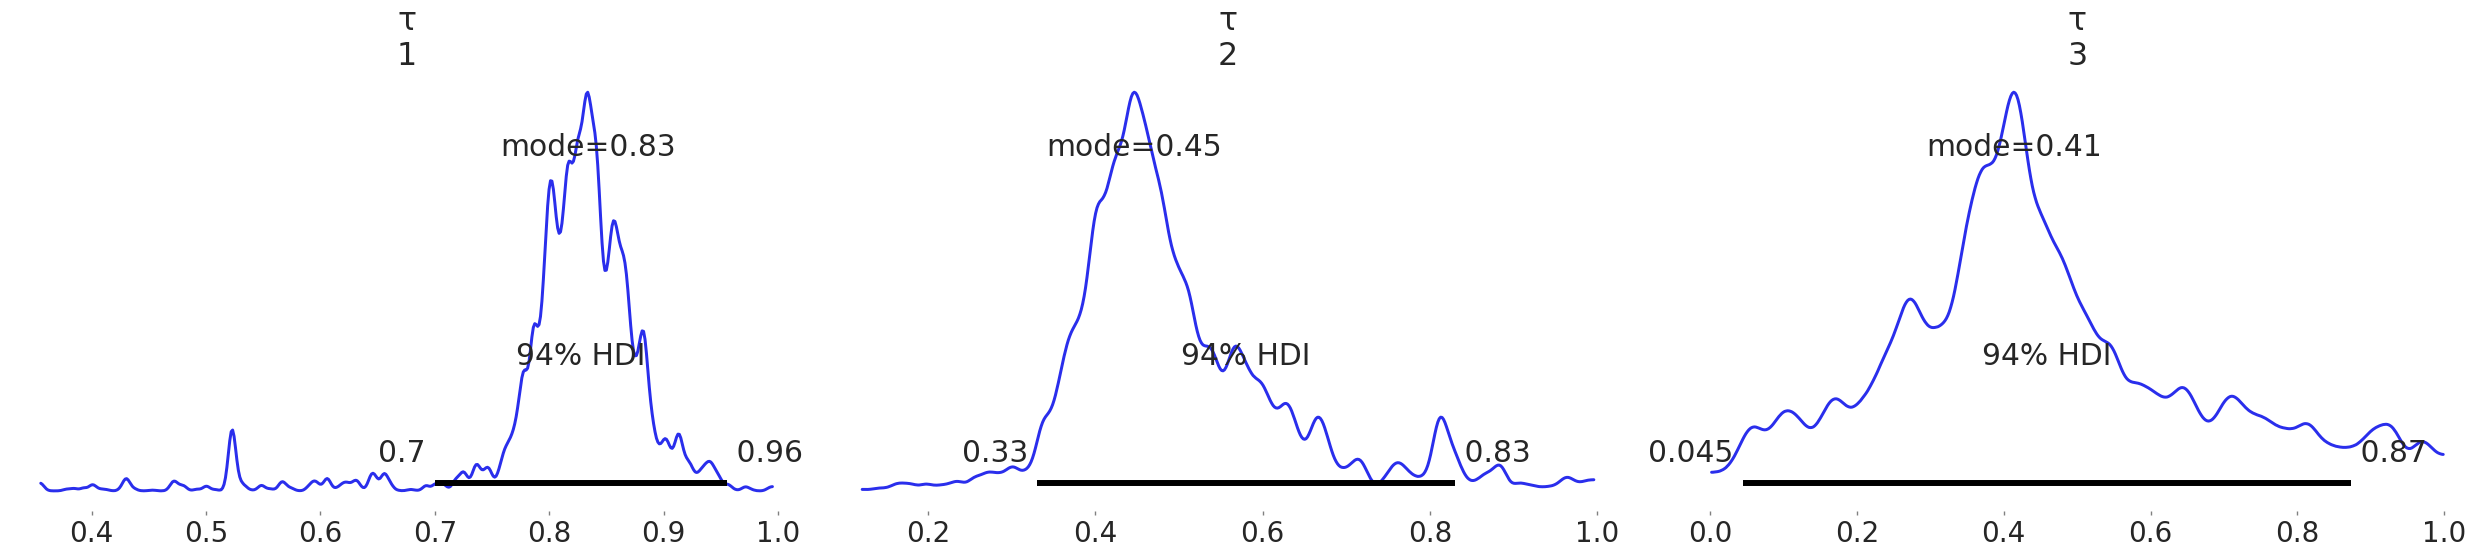
\includegraphics[width=.9\textwidth]{credible_intervals}}
  \caption{Example of 94\% credible intervals on the posterior distribution of the impact points.}\label{fig:credible_intervals}
\end{figure}


Moreover, we can perform various visual checks, such as a plot comparing both the observed and posterior predictive distribution of the responses (see Figure~\ref{fig:ppc}). The posterior predictive distribution for a new sample \(x\) is formally defined as
\[
\pi(y\mid x, \mathcal D_n) = \int_{\Theta} \pi(y\mid x, \theta)\pi(\theta\mid \mathcal D_n)\, d\theta,
\]
and in our context it can be approximated by the simulated responses \(\symbf Y^* \equiv \{\symbf Y^{(m)*}\}\), following the notation of~\eqref{eq:sampled-response-vector}. This distribution accounts for the uncertainty about \(\theta\), and we do indeed use it for prediction in our predict-then-summarize approach.

\begin{figure}[ht!]
  \centering
  \setlength{\fboxrule}{.5pt}%
  \fbox{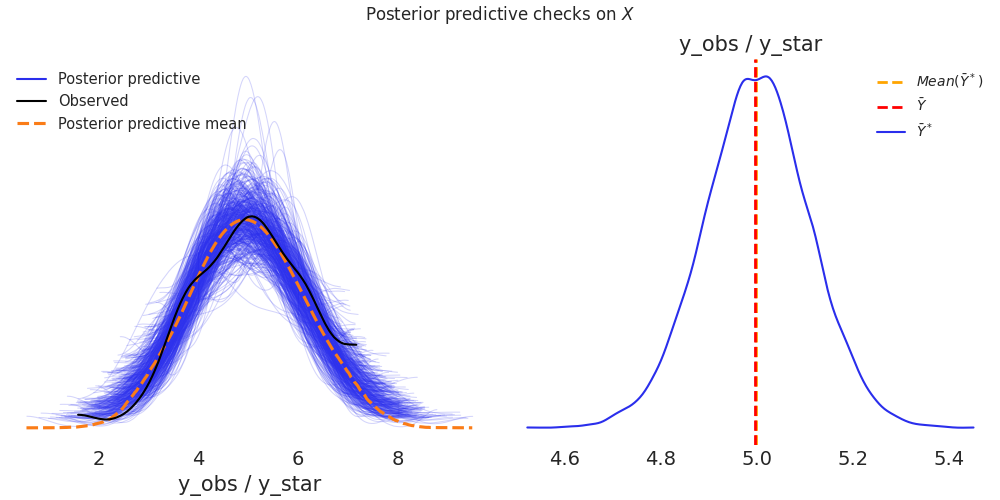
\includegraphics[width=.65\textwidth]{ppc_linear}}
  \caption{Example of posterior predictive graphical checks on a fitted linear regression model. We show a comparison between the observed distribution of the response variable and the posterior predictive distribution consisting on the approximate sampled responses.}\label{fig:ppc}
\end{figure}


In addition, we can calculate the so-called \textit{Bayesian p-values} for several statistics, which are defined as \(P(T(\symbf Y^*)\leq T(\symbf Y)| \symbf Y)\), and are computed by simply measuring the proportion of the \(M\) estimates \(T\{\symbf Y^{(m)*}\}\) that fall below the observed value of the statistic, \(T(\symbf{Y})\). They are expected to be around 0.5 when the model accurately represents the data, and a deviation either way can be indicative of modeling issues; see Chapter 6 of \citet{gelman2013bayesian} for details.

%%%%%%%%%%%%%%%%%%%%%%%%%%%%%%%%%%%%%%%%%%%%%%%%%%%%%%%%%%%%%%%%%%%%%%%%
% Copyright (c) 2022 Antonio Coín
%
% This work is licensed under a
% Creative Commons Attribution-ShareAlike 4.0 International License.
%
% You should have received a copy of the license along with this
% work. If not, see <http://creativecommons.org/licenses/by-sa/4.0/>.
%%%%%%%%%%%%%%%%%%%%%%%%%%%%%%%%%%%%%%%%%%%%%%%%%%%%%%%%%%%%%%%%%%%%%%%%

\let\epsilon\varepsilon

%%%%%%%%%%%%%%%%%%%%%%%%%%%%%%%%%%%%%%%%%%%%%%%%%%%%%%%%%%%%%%%%%%%%%%%%
\chapter{Experiments}\label{ch:experiments}
%%%%%%%%%%%%%%%%%%%%%%%%%%%%%%%%%%%%%%%%%%%%%%%%%%%%%%%%%%%%%%%%%%%%%%%%

In this chapter we present the results of the experiments carried out to test the performance of our models in different scenarios, both simulated and with real data. The structure of the code and other minor computational details are discussed in Appendix~\ref{ch:code}.

\subsection*{Experimental setting}

First and foremost, we consider \(T=\{\text{mean, median, mode}\}\) for our summarize-then-predict approach to prediction (see~\eqref{eq:summarize-predict-linear} and~\eqref{eq:summarize-predict-logistic}). As a result, in linear regression we have 4 prediction methods (one for each statistic and one for the predict-then-summarize approach) and 3 variable selection methods (one for each statistic), while in logistic regression there are similarly 5 prediction methods and 3 variable selection procedures. In each case, after variable selection is performed, we use a \(l^2\)-penalized multiple linear/logistic regression method to generate the corresponding predictions. All in all, we are looking at 7 (8 in the case of logistic regression) prediction methods, and although all of them are derived from a single MCMC run, we will treat them as separate for the purposes of the experimentation. In what follows we relax the notation and use the expressions ``model'', ``prediction method'' and ``algorithm'' almost interchangeably when referring to these 7 (or 8) cases.

We consider \(n=150\) training samples and \(n'=100\) testing samples on an equispaced grid of \(N=100\) points on \([0, 1]\) for the simulated data sets, and we do a 66\%/33\% train/test split on the real data sets. We then perform \(5\)-fold cross validation (CV) on the training set to select the best values of \(p\) and \(\eta\) for each model, and after refitting the best model in each case on the whole training set, we evaluate it and measure the predictive performance on the test set. We look for \(p\) in the set \(\{1,2,\dots,10\}\), while the possible values of \(\eta\) are \(\{10^{-4}, 10^{-3}, \dots, 10^2\}\).

Because of execution time constraints, the hyperparameters of the MCMC method are not part of the CV process, and are selected manually based on an initial set of experiments, as well as recommendations from the original article. We use 64 chains and run them for 900 iterations in total, discarding the first 500 iterations as burn-in. Moreover, we use a weighted mixture of walk and stretch moves in the \textit{emcee} sampler to advance the chains in each iteration, selecting the stretch move (the default) with probability 0.7 or the walk move with probability 0.3.

Lastly, since the use of MCMC algorithms introduces a source of stochasticity in the prediction procedure, we independently repeat the whole process 10 times (each with a different train/test configuration), and average the results across these executions. The metrics used to evaluate the performance of the models are the RMSE for linear regression and the accuracy for logistic regression. Recall that
\[
\operatorname{RMSE}(\{\hat y_i\}) = \sqrt{\frac{1}{n'}\sum_{i=1}^{n'} (y_i - \hat y_i)^2}
\]
and
\[
\operatorname{Accuracy}(\{\hat y_i\}) = \frac{1}{n'} \sum_{i=1}^{n'} \I(y_i = \hat y_i).
\]

\subsection*{Data sets}

We consider a set of functional regressors common to linear and logistic regression problems. They are four Gaussian processes (GP's), each with a different covariance function:
\begin{enumerate}
  \item BM.\hspace{0.3em} A Brownian motion \(K_1(t,s)=\min\{t,s\}\).
  \item fBM.\hspace{0.3em} A fractional Brownian motion \(K_2(t,s)=1/2(s^{2H} + t^{2H} - |t-s|^{2H})\), with Hurst parameter \(H=0.8\).
  \item O-U.\hspace{0.3em} An Ornstein-Uhlenbeck process \(K_3(t,s)=e^{-|t-s|}\).
  \item Gaussian.\hspace{0.3em} A Gaussian process with Gaussian kernel \(K_4(t,s)=e^{-(t-s)^2/2\nu^2}\), where \(\nu=0.2\).
\end{enumerate}
Also, when applicable, we fix a variance \(\sigma^2=0.5\) for the error terms \(\epsilon\).

\paragraph{Linear regression data sets.} We consider three different types of simulated data sets, all with a common value of \(\alpha_0=5\).
\begin{itemize}
  \item A finite-dimensional RKHS model where the response is generated as \(Y=5 -5X(0.1) + X(0.4) + 10X(0.8) + \epsilon\), for each of the four GP's mentioned above.
  \item A \(L^2\)-model with underlying coefficient function \(\beta(t)=\log(1+4t)\), again for the same four GP's.
  \item A model based on non-GP regressors. Specifically, we use a geometric Brownian motion (GBM) defined as \(X(t)=e^{BM(t)}\), where \(BM(t)\) is a standard Brownian motion. In this case we consider two data sets, one with a RKHS response and one with a \(L^2\) response, with the same parameters as above.
\end{itemize}
As for the real data sets, we use the (twice-differentiated) Tecator data set introduced in Chapter~\ref{ch:introduction} to predict fat content of 193 meat samples, as well as what we call the Moisture \citep{kalivas1997two} and Sugar \citep{bro1999exploratory} data sets. The first consists of near-infrared spectra of 100 wheat samples and the objective is to predict the samples' moisture content, whereas the second contains 268 samples of sugar fluorescence data in order to predict ash content. The three data sets are measured on a grid of 100, 101 and 115 equispaced points on \([0, 1]\), respectively.

\paragraph{Logistic regression data sets.} Again we consider three different types of simulated data sets,  with a common value of \(\alpha_0=-0.5\). In this case we randomly permute 10\% of the labels to introduce some noise in the simulations.
\begin{itemize}
  \item Four logistic finite-dimensional RKHS models with the same functional parameter as in the linear regression case (one for each GP). Specifically,
  \[
  \P(Y=1\mid X) = \frac{1}{1 + \exp\left\{0.5 +5X(0.1) - X(0.4) - 10X(0.8)\right\}}.
  \]
  \item Four logistic \(L^2\)-models with the same coefficient function as in the linear regression case, i.e.:
  \[
  \P(Y=1\mid X) = \frac{1}{\displaystyle 1 + \exp\left\{0.5 - \int_0^1 \log(1+4t) X(t)\, dt\right\}}.
  \]
  \item A ``mixture'' model based on non-GP regressors, in which we mix regressors from two different GP's (with equal probability \(p=1/2\)) and label them according to their origin. Firstly, we consider a homoscedastic case to distinguish between a standard Brownian motion and a Brownian motion with a mean function that is zero until \(t=0.5\), and then becomes \(m(t)=0.75t\). Secondly, we consider a heteroscedastic case to distinguish between a standard Brownian motion and a Brownian motion with variance 2, that is, with kernel \(K(t,s)=2\min\{t,s\}\).
\end{itemize}
Additionally, we use three real data sets well known in the literature. The first one is a subset of the Medflies data set \citep{carey1998relationship}, consisting on samples of the number of eggs laid daily by 534 flies over 30 days, to predict if their longevity is high or low. The second one is the Berkeley Growth Study data set \citep{tuddenham1954physical}, which records the height of 54 girls and 39 boys over 31 different points in their lives. Finally, we selected a subset of the Phoneme data set \citep{hastie1995penalized}, based on 200 digitized speech frames over 128 equispaced points to predict the phonemes ``aa'' and ``ao''.

\subsection*{Comparison algorithms}

We have included a fairly comprehensive suite of comparison algorithms, chosen among the most common methods used in machine learning and FDA. There are purely functional methods, finite-dimensional models that work on the discretized data, and variable selection/dimension reduction procedures.

\paragraph{Linear regression comparison algorithms.} We consider the following regression methods:
\begin{itemize}
  \item Manual.\hspace{.3em} Dummy variable selection method with a pre-specified number of components (equispaced on \([0, 1]\)).
  \item Lasso.\hspace{.3em} Linear least squares with \(l^1\) regularization.
  \item Ridge.\hspace{.3em} Linear least squares with \(l^2\) regularization.
  \item PLS.\hspace{.3em} Partial least squares for dimension reduction.
  \item PCA.\hspace{.3em} Principal component analysis for dimension reduction.
  \item PLS1.\hspace{.3em} Partial least squares regression \citep[e.g.][]{wegelin2000survey}.
  \item APLS.\hspace{.3em} Functional partial least squares regression proposed by \citet{delaigle2012methodology}.
  \item RMH.\hspace{.3em} Recursive maxima hunting variable selection method proposed by \citet{torrecilla2016feature}.
  \item FLin.\hspace{.3em} Functional \(L^2\) linear regression model with fixed basis expansion.
  \item FPCA.\hspace{.3em} Functional principal component analysis.
  \item FPLS1.\hspace{.3em} Functional PLS regression through basis expansion, implemented as in \citet{aguilera2010using}.
\end{itemize}

\paragraph{Logistic regression comparison algorithms.} All the variable selection and dimension reduction algorithms from above are also considered in this case, plus the following classification methods:
\begin{itemize}
  \item Log.\hspace{.3em} Standard multiple logistic regression with \(l^2\) regularization.
  \item LDA.\hspace{.3em} Linear discriminant analysis.
  \item QDA.\hspace{.3em} Quadratic discriminant analysis.
  \item RKVS.\hspace{.3em} RKHS-based variable selection method proposed in \citet{berrendero2018use}.
  \item APLS.\hspace{.3em} Functional PLS used as a dimension reduction method, as proposed in \citet{delaigle2012achieving} in combination with the nearest centroid (NC) algorithm.
  \item FLog.\hspace{.3em} Functional RKHS-based logistic regression algorithm proposed in \citet{berrendero2018functional}.
  \item FLDA.\hspace{.3em} Implementation of the functional version of linear discriminant analysis proposed in \citet{preda2007pls}.
  \item MDC.\hspace{.3em} Maximum depth classifier \citep[e.g.][]{ghosh2005maximum}.
  \item FKNN.\hspace{.3em} Functional K-nearest neighbors classifier with the \(L^2\)-distance.
  \item FNC.\hspace{.3em} Functional nearest centroid classifier with the \(L^2\)-distance.
\end{itemize}

The main parameters of all these algorithms are selected by cross-validation, using the same 5 folds as our proposed models so that the comparisons are fair. In particular, regularization parameters are searched among 20 values in the logarithmic space \([10^{-4}, 10^4]\), the number of manually selected variables is one of \(\{5, 10, 15, 20, 25, 50\}\), the number of components for dimension reduction and variable selection techniques is in the set \(\{2, 3, 4, 5, 7, 10, 15, 20\}\), the number of basis elements for cubic spline bases is in \(\{8,10,12,14,16\}\), the number of basis elements for Fourier bases is one of \(\{3,5,7,9,11\}\), and the number of neighbors in the KNN classifier is in \(\{3,5,7,9,11\}\).

Most algorithms have been taken from the libraries \textit{scikit-learn}\footnote{\url{https://scikit-learn.org}} and \textit{scikit-fda}\footnote{\url{https://fda.readthedocs.io}}, the first oriented to machine learning in general and the second to functional data analysis in particular. However, some methods were not found in these packages and had to be implemented from scratch. This is the case of the FLDA, FPLS and APLS methods, which we coded following the corresponding articles.

\subsection*{Results display}

We have adopted a visual approach to presenting the experimentation results, using colored graphs to help visualize them. We felt that this was a better way of summarizing a large empirical study such as the one we have carried out. Alternatively, tables representing these results can be consulted in Appendix~\ref{ch:tables}.

We show the mean and standard deviation of the score obtained in each case across the 10 random runs, depicting our models in orange and the comparison algorithms in blue. We also show the global mean of all the comparison algorithms with a dashed vertical line, and we exclude extreme negative results from this mean to avoid distortion. Moreover, we separate complete prediction algorithms from two-stage methods, the latter being the ones that perform variable selection or dimension reduction prior to a multiple linear/logistic regression method.

We do not expect our models to defeat all the comparison algorithms in all cases (and indeed they do not), but we intend to show that they are competitive methods that on average match or improve the performance of other usual alternatives. After all, \textit{there is no such thing as a free lunch}\footnote{The phrase alludes to the No Free Lunch theorem, which loosely speaking asserts that all machine learning methods are equivalent when their performance is averaged across all possible problems. However, the practical implications of this statement are questionable \citep[see e.g.][]{giraud2005toward}.}!

\section{Functional linear regression}\label{sec:experiments-linear}

\subsection*{Simulated data sets}

In Figure~\ref{fig:reg_emcee_rkhs} we see the results for the four GP regressors considered in the RKHS case. This is the most favorable case for us, as the underlying model coincides with our assumed model. Indeed, we can see that in most cases our algorithms are the ones with lower RMSE, save for a few exceptions, notably the Gaussian kernel. A subsequent analysis showed that this particular data set is especially sensitive to the value of the hyperparameter \(\eta\) in our prior distribution, so a more customized approach would be needed to obtain better results.

\vspace{.3em}

\begin{figure}[ht!]
  \centering
  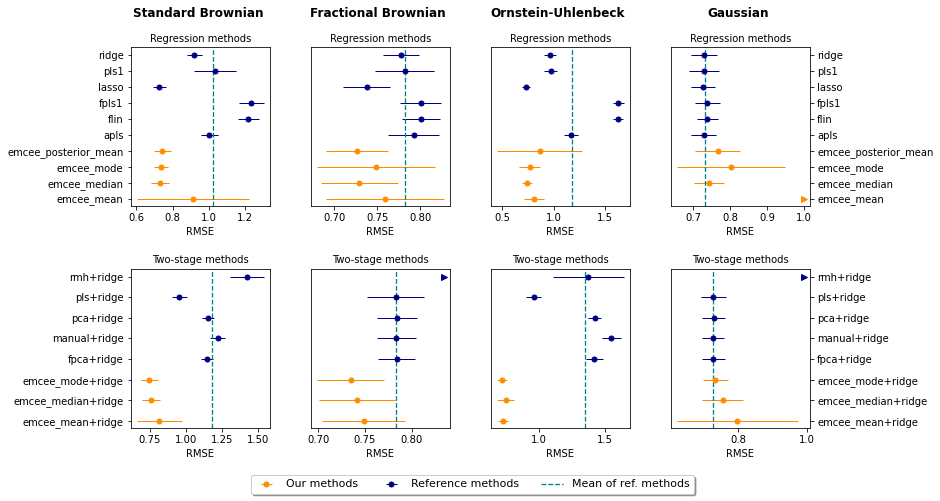
\includegraphics[width=\textwidth]{reg_emcee_rkhs}
  \caption{RMSE of predictors for simulated GP data that obeys an underlying RKHS model (lower is better).}\label{fig:reg_emcee_rkhs}
\end{figure}

In Figure~\ref{fig:reg_emcee_l2} we see the results for the case with an underlying \(L^2\)-model, which would be our most direct competitor. In this case the outcome is satisfactory, since for the most part our models are on a par with the rest, even beating other methods that were designed with the \(L^2\)-model in mind. Moreover, whenever one of our models has a higher RMSE, the difference is pretty small in comparison. Note that some of our Bayesian models have a higher standard deviation, partly because there is an intrinsic randomness in the methods (apart from the train/test splits), and it can be the cause of the occasional worse performance. In relation to this, we observe that the methods that use the mean as a summary statistic tend to perform much worse. This is because the mean is very sensitive to outliers, so if at some point there is a chain that randomly deviates from the rest, the mean of the posterior distribution will be greatly impacted. In particular, very high values of the parameter \(\sigma^2\) were reported sometimes, producing misleading results when averaged with the rest of the values.

\enlargethispage{1\baselineskip}

Lastly, the results for the non-GP case can be seen in Figure~\ref{fig:reg_emcee_nongp}, in which the regressors are realizations of a GBM. In this case we still get better results under the RKHS model, while the results under the \(L^2\)-model are slightly worse. However, as before, the difference is small (except for the \textit{emcee\_mean} methods).

\vspace{.2em}

\begin{figure}[ht!]
  \centering
  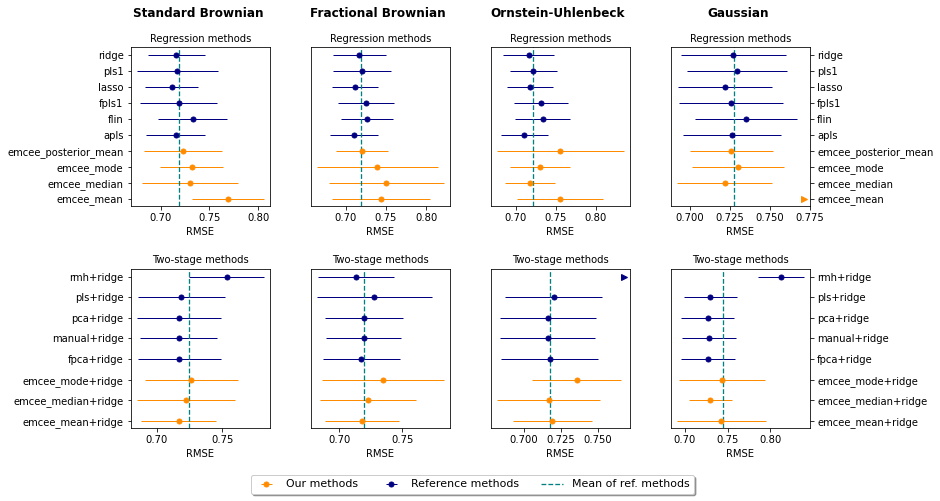
\includegraphics[width=\textwidth]{reg_emcee_l2}
  \caption{RMSE of predictors for simulated GP data that obeys an underlying \(L^2\) model (lower is better).}\label{fig:reg_emcee_l2}
\end{figure}

\begin{figure}[ht!]
  \centering
  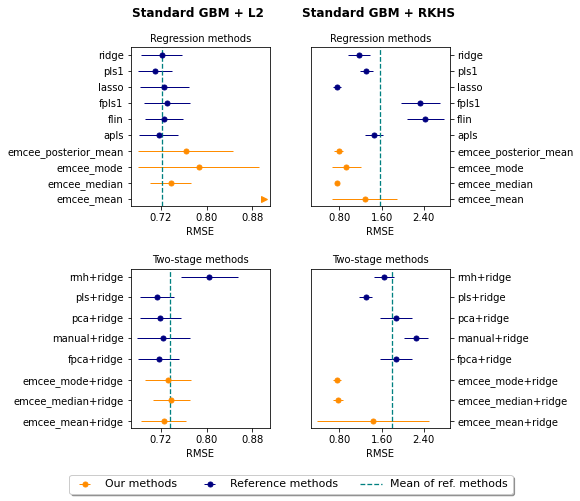
\includegraphics[width=.65\textwidth]{reg_emcee_nongp}
  \caption{RMSE of predictors for simulated data with GBM regressors (lower is better).}\label{fig:reg_emcee_nongp}
\end{figure}

\subsection*{Real data}

Figure~\ref{fig:reg_emcee_real} shows the results for the real data sets. In these data sets there is a substantial difference in performance between some of our methods and the reference algorithms. However, the predict-then-summarize approach (represented as \textit{posterior\_mean}) seems to work quite well, always scoring near the mean RMSE of all the comparison algorithms. Moreover, our two-stage methods seem to outperform the summarize-then-predict methods in these cases, scoring again very close to the mean of the reference methods.

We have to bear in mind that real data is more complex and noisy than simulated data, and it is possible that after a suitable pre-preprocessing we would obtain better results with our methods. However, our goal was to perform a general comparison without focusing too much on the specifics of any particular data set.

\begin{figure}[ht!]
  \centering
  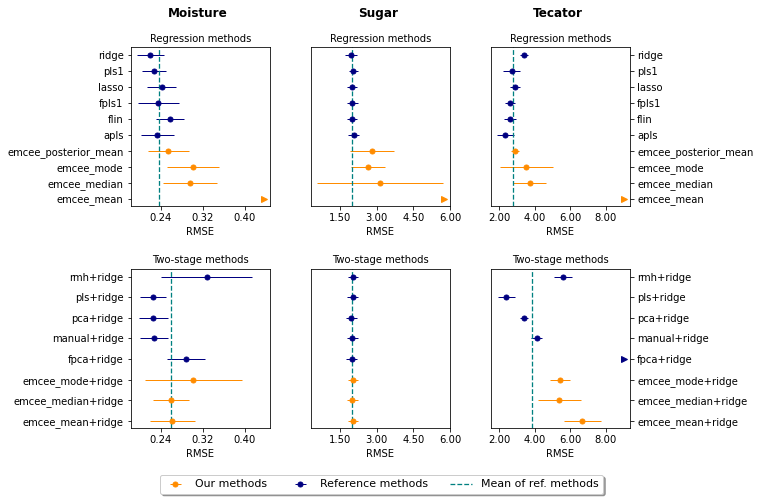
\includegraphics[width=.85\textwidth]{reg_emcee_real}
  \caption{RMSE of predictors for real data sets (lower is better).}\label{fig:reg_emcee_real}
\end{figure}

\section{Functional logistic regression}\label{sec:experiments-logistic}

\subsection*{Simulated data sets}

In Figure~\ref{fig:clf_emcee_rkhs} we see the results for the GP regressors in the logistic RKHS case. Our models perform fairly well in this advantageous case, although the two-stage methods fare somewhat poorly in these data sets. However, in most cases the differences observed account for only one or two misclassified samples.

\begin{figure}[ht!]
  \centering
  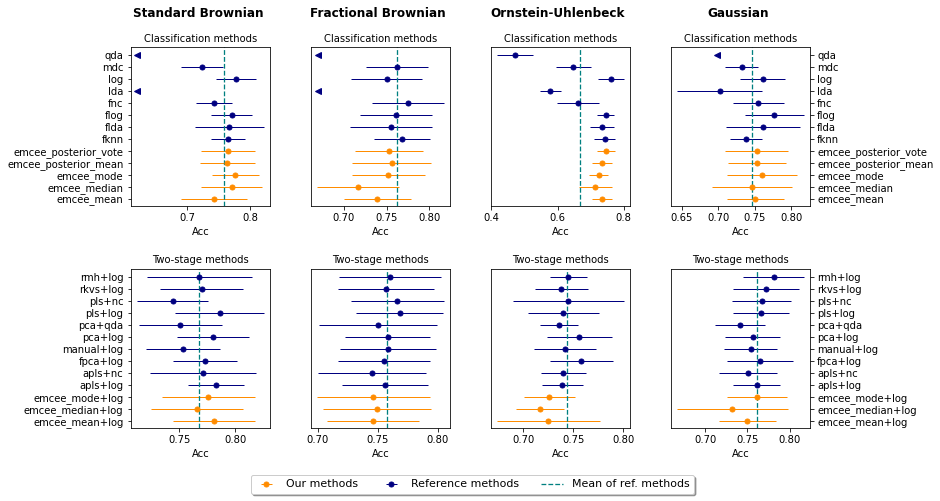
\includegraphics[width=\textwidth]{clf_emcee_rkhs}
  \caption{Accuracy of classifiers for simulated GP data that obeys an underlying logistic RKHS model (higher is better).}\label{fig:clf_emcee_rkhs}
\end{figure}

Continuing with Figure~\ref{fig:clf_emcee_l2}, we see that in the \(L^2\) case the results are again promising, since our models score consistently on or above the mean of the reference models, and in many cases surpassing most of them. The predict-then-summarize approaches (\textit{emcee\_posterior\_mean} and \textit{emcee\_posterior\_vote}) are particularly good in this case, and in general have low standard errors. Moreover, the overall accuracy of all methods is low (below 60\%), so this is indeed a difficult problem in which even small increases in accuracy are relevant.

Finally, Figure~\ref{fig:clf_emcee_nongp} shows that our classifiers perform better than most comparison algorithms when separating two homoscedastic Gaussian processes, but they struggle in the heteroscedastic case. Incidentally, this heteroscedastic case of two zero-mean Brownian motions has a special interest, since it can be shown that the Bayes error is zero in the limit of dense monitoring (i.e. with an arbitrarily fine measurement grid), a manifestation of the ``near-perfect'' classification phenomenon analyzed for example in \citet{torrecilla2020optimal}. Our results are in line with the empirical studies of this article, where the authors conclude that even though the asymptotic theoretical error is zero, most classification methods are suboptimal in practice (possibly due to the high collinearity of the data), with the notable exception of PCA+QDA.

\begin{figure}[htbp!]
  \centering
  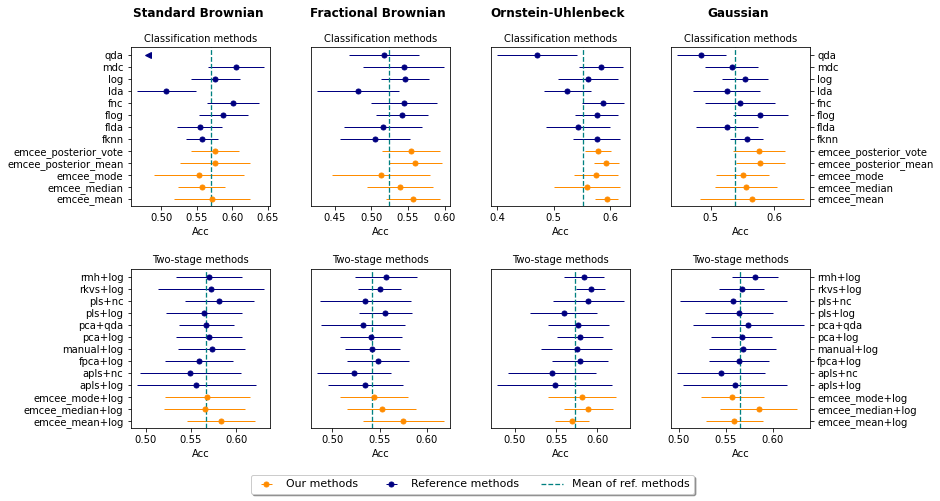
\includegraphics[width=\textwidth]{clf_emcee_l2}
  \caption{Accuracy of classifiers for simulated GP data that obeys an underlying logistic \(L^2\)-model (higher is better).}\label{fig:clf_emcee_l2}
\end{figure}

\begin{figure}[htbp!]
  \centering
  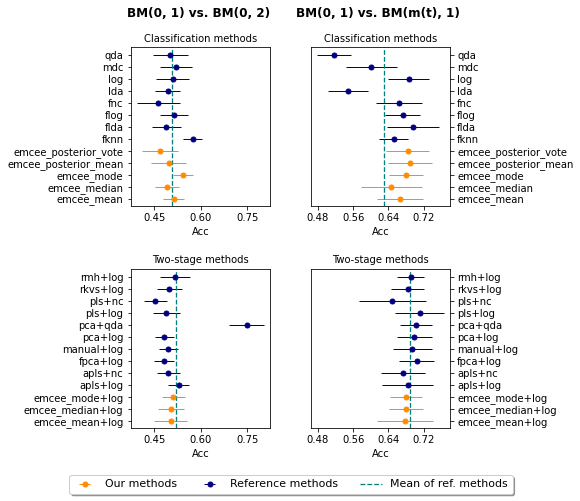
\includegraphics[width=.65\textwidth]{clf_emcee_nongp}
  \caption{Accuracy of classifiers for simulated data coming from two different GP's, labeled according to their origin (higher is better).}\label{fig:clf_emcee_nongp}
\end{figure}

\subsection*{Real data}

As for the real data sets, in Figure~\ref{fig:clf_emcee_real} we see positive results in general, obtaining in most cases accuracies well above the mean of the reference models, and sometimes above most of them. In particular, the predict-then-summarize methods tend to have a good performance and achieve a lower standard error across executions, which is a trend that we also saw in the simulated data sets. However, our variable selection methods seem to be a bit worse in this case. Again, the models that use \textit{emcee\_mean} are the exception, and in all these data sets they perform steadily worse than the rest of our Bayesian models.

\begin{figure}[ht!]
  \centering
  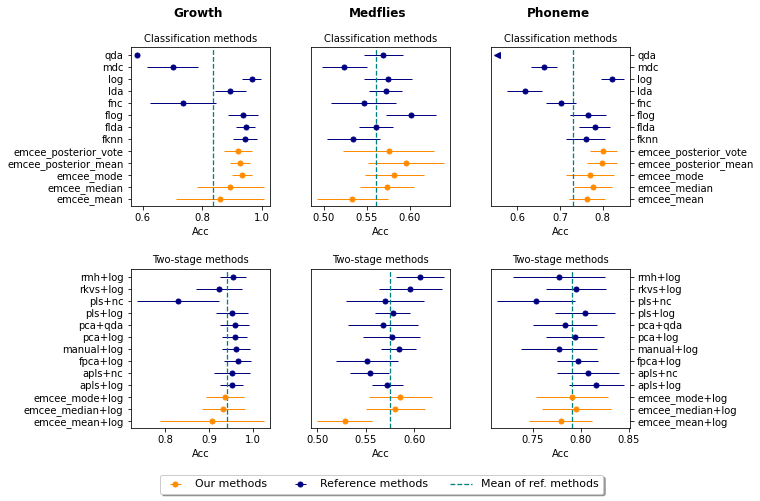
\includegraphics[width=.85\textwidth]{clf_emcee_real}
  \caption{Accuracy of classifiers for real data sets (higher is better).}\label{fig:clf_emcee_real}
\end{figure}


\section{Additional experiments}

In this section we present some experiments that are not directly related to measuring the predictive performance of our models relative to other methods.

\subsection*{Model misspecification}

One requirement that our model should satisfy is that it ought to be able to recover the true parameter function when the underlying data generation model is a finite-dimensional RKHS model. This is generally the case when the value of \(p\) in our model and the true value of \(p\) coincide, but what happens when we change the value of \(p\) in the model?

Take for example a RKHS data set with two components generated according to the formula \(Y=5 -5X(0.1) + 10X(0.8) + \epsilon\), with \(\epsilon\sim \mathcal N(0, 0.5)\). Figure~\ref{fig:beta_trace_3} shows the resulting posterior distribution of the parameters \(b=(\beta_1, \beta_2, \beta_3)\) and \(\tau=(t_1, t_2, t_3)\) for a model with 3 components. As we can see, one of the coefficients has gone to zero to account for the overspecification of the model, while the other two have stabilized very close to the true parameters. The same goes for the time instants, except that in this case there is no default value to represent that a component is unused, so the time corresponding to the null coefficient oscillates back and forth. The estimated function (based for example in the mode of the posterior distributions) will not be perfect, essentially because of the noise in the response. But it should be close to the true parameter function \(\alpha(t)=-5K(t, 0.1) + 10K(t, 0.8)\), providing a good predictive performance.

\begin{figure}[ht!]
  \centering
  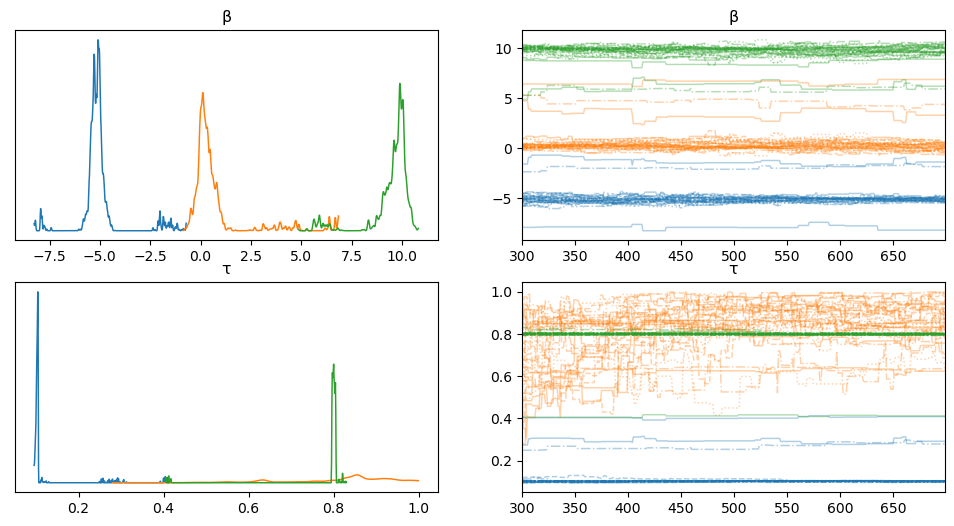
\includegraphics[width=.8\textwidth]{beta_trace_3}
  \caption{Estimated posterior distribution for \(b\) and \(\tau\) in a linear model with \(p=3\) (left) and the corresponding trace evolution for 400 iterations in the MCMC sampler (right).}\label{fig:beta_trace_3}
\end{figure}

In contrast, if we consider now a model with \(p=4\) with the same data, we might obtain posterior distributions like the ones in Figure~\ref{fig:beta_trace_4}. In this situation two coefficients should go to zero, but that is no longer the case. For example, while the green component has a high density around 0, it also has a considerable mass around 10, effectively ``competing'' with the red component. This is a manifestation of the label switching issue, caused in this case by an excessive number of degrees of freedom in the model.

\begin{figure}[ht!]
  \centering
  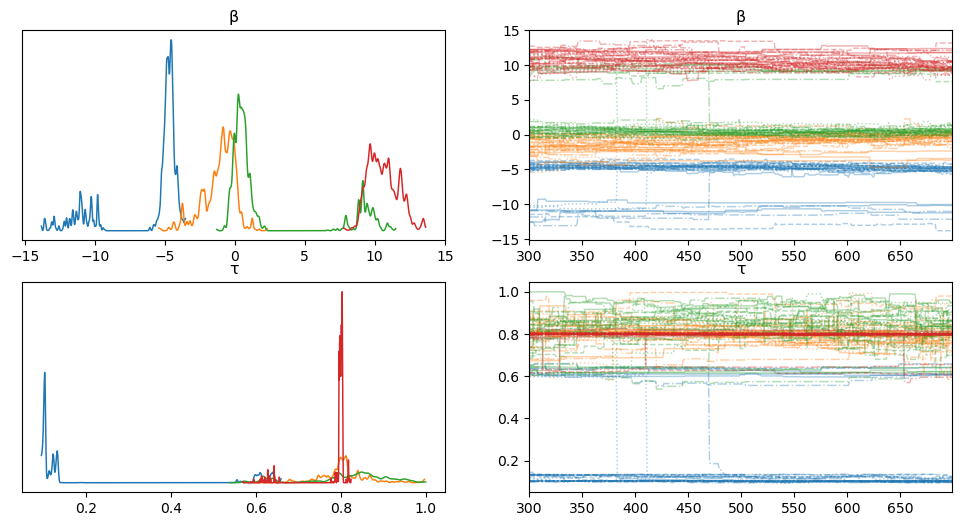
\includegraphics[width=.8\textwidth]{beta_trace_4}
  \caption{Estimated posterior distribution for \(b\) and \(\tau\) in a linear model with \(p=4\) (left) and the corresponding trace evolution for 400 iterations in the MCMC sampler (right).}\label{fig:beta_trace_4}
\end{figure}

There is still another possible situation, one in which there is no label switching but the estimated function has four non-negligible components. This can happen because the different components exploit the additional freedom and ``work together'', so to speak. In this way we might obtain an estimate that does not resemble the true coefficient function, but that has a very low prediction error. However, this could also work to our detriment and cause the estimated function to be worse prediction-wise than simpler alternatives. This phenomenon is expected to strengthen as the difference between the true and assumed value of \(p\) grows larger.

\subsection*{Dependence on \(p\)}

Another thing we wanted to look at was the dependence of the final prediction result on the chosen value of \(p\), especially when there is no concept of ``components'' in the underlying model. We can take for example the homoscedastic mixture data set described earlier for the logistic regression problem, and fix the parameter \(\eta=0.01\). The corresponding mean accuracies (in 10 repetitions) for RKHS models with \(p=1,2,\dots 10\) components are shown in Figure~\ref{fig:dependence_acc_p}, along with their standard errors (which are arguably not very informative).

\begin{figure}[ht!]
  \centering
  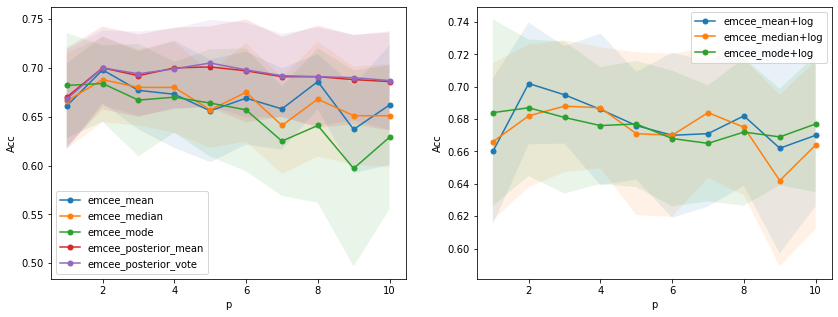
\includegraphics[width=0.9\textwidth]{mixture_dependence_acc_p}
  \caption{Mean accuracy in 10 repetitions for our logistic RKHS methods as a function of \(p\), using \(\eta=0.01\) and the homoscedastic mixture data set. The corresponding standard errors are shown in faded colors.}\label{fig:dependence_acc_p}
\end{figure}

It would appear that the methods that use the whole posterior distribution are more stable and somewhat independent of the value of \(p>1\). The other algorithms show a slight downward trend as \(p\) increases (although not so much in the variable selection methods), and in general their best results are obtained at \(p=2\) and \(p=8\). We expect that this effect or some small variation of it will remain valid in other situations; however, a profound study of this would be the subject of a different experiment altogether.

\subsection*{Execution times}

We summarize below the mean execution time for each independent run of our CV experiment, grouping the simulated data sets by the underlying data generation strategy (since the results within these groups were very similar).

\begin{table}[ht!]
  \centering
  \begin{tabular}{lcccccc}
\toprule
  &            RKHS &           \(L^2\) &           GBM &        Tecator & Moisture & Sugar \\
\midrule
Linear regression & 260 & 245 & 264 & 230 & 264 & 285\\
\bottomrule

  &            RKHS &           \(L^2\) &           Mixture &        Medflies & Growth & Phoneme \\
\toprule
Logistic regression & 277 & 263 & 246 & 250 & 218 & 277\\
\bottomrule
\end{tabular}
  \caption{Mean execution times (in minutes) for the independent runs of the CV experiments in Sections~\ref{sec:experiments-linear} and~\ref{sec:experiments-logistic}, grouped when possible by the underlying data generation strategy.}
\end{table}

The reference algorithms used were all fast methods that can complete their whole CV loop in just a few seconds, so any comparison with them in this regard is uninteresting. However, this outcome was to be expected, since in general the MCMC methods are known to have a high computational cost in exchange for the simplicity in modeling they provide. An individual MCMC run is not that expensive time-wise, but even for a modest 5-fold cross-validation loop the effects add up quickly to a considerable amount of time. In Figure~\ref{fig:dependence_time_n_train} we show the evolution of the execution time (in seconds) versus the number of training samples in a generic case, which not surprisingly has a more or less linear behavior. This, however, is not an impediment for using our methods in practice.

\begin{figure}[ht!]
  \centering
  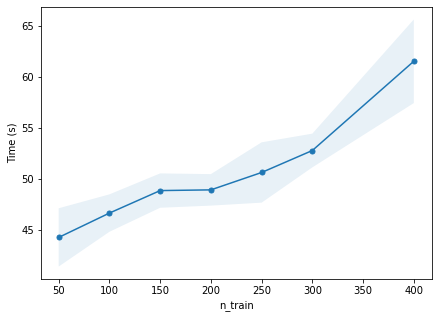
\includegraphics[width=0.55\textwidth]{l2_dependence_time_n_train}
  \caption{Mean training times of a logistic RKHS model with \(p=5\), as a function of the number of training samples (averaged across 10 independent runs). The values are surrounded by their corresponding standard deviations.}\label{fig:dependence_time_n_train}
\end{figure}

\subsection*{Non-reported experiments}

Apart from all the experiments described above, we performed several tests with different configurations and alternatives. Although these trials did not produce better results in general, we mention some of them here to show how the model could be easily extended. In fact, most of these modifications, if not all, are still available in the provided code and can be enabled through specific parameters.

The first thing we tried was to make the parameter \(p\) part of the Bayesian model, imposing a categorical prior distribution on it. As explained in Chapter~\ref{ch:model-choice}, this approach led to many complications and generally poor results. However, the idea of letting the model select how many components it should have based on the data is an interesting one, and in some situations this could greatly improve the results of variable selection procedures based on other model selection criteria.

We also tried changing some prior distributions. For instance, we swapped the improper prior distribution on \(\sigma^2\) for a Cauchy distribution on \(\R^+\). The results were similar, but we ultimately discarded this approach because it introduced yet another hyperparameter into the model with no clear benefit. In addition, we tried to impose a beta distribution on each of the time instants \(t_j\), selecting the corresponding shape parameters in a semi-automatic way so that most of the density fell in the areas where the variance of the process was higher (and thus the effect of individual trajectories was more noticeable). This approach does work, but in our estimation the computational overhead introduced by the beta density function (sometimes resulting in a 1.5x increase in execution time) is not worth the mild improvements, if any.

A lot of minor things were tried, such as standardizing the regressors and/or the responses, smoothing the functional data, changing the proposal of moves in the MCMC sampler, or transforming the values of \(\tau\) during sampling so that the domain was unconstrained. It is likely that some of these strategies would lead to better results in specific cases, but overall they did not improve the general performance of the prediction procedure.

%%%%%%%%%%%%%%%%%%%%%%%%%%%%%%%%%%%%%%%%%%%%%%%%%%%%%%%%%%%%%%%%%%%%%%%%
% Copyright (c) 2022 Antonio Coín
%
% This work is licensed under a
% Creative Commons Attribution-ShareAlike 4.0 International License.
%
% You should have received a copy of the license along with this
% work. If not, see <http://creativecommons.org/licenses/by-sa/4.0/>.
%%%%%%%%%%%%%%%%%%%%%%%%%%%%%%%%%%%%%%%%%%%%%%%%%%%%%%%%%%%%%%%%%%%%%%%%

%%%%%%%%%%%%%%%%%%%%%%%%%%%%%%%%%%%%%%%%%%%%%%%%%%%%%%%%%%%%%%%%%%%%%%%%
\chapter{Conclusions}\label{ch:conclusions}
%%%%%%%%%%%%%%%%%%%%%%%%%%%%%%%%%%%%%%%%%%%%%%%%%%%%%%%%%%%%%%%%%%%%%%%%

\begin{outcomment}
  Algo que no he comentado en ninguna parte es que el tiempo de ejecución de nuestros modelos es bastante alto (del orden de 30-40 segundos por ejecución) frente al de los algoritmos de comparación (unos pocos segundos en general). Como es algo negativo, no sé muy bien cómo ponerlo, si comentarlo de pasada aquí en las conclusiones, o dedicarle un poco más de espacio en el capítulo de experimentos.\\
\end{outcomment}

\begin{outcomment}
  Algunos comentarios generales:
  \begin{itemize}
    \item Destacar las ventajas de lo bayesiano: flexibilidad, incorporación de información con distintas priors, etc.
    \item Destacar la interpretabilidad y sencillez de nuestro modelo. En general, conseguimos resultados competitivos usando modelos con baja dimensión.
    \item Los resultados en regresión logística parecen en media un poco mejores que en regresión lineal.
    \item No se recomienda usar la media como estadístico de resumen de la distribución a posteriori.
    \item La búsqueda de hiperparámetros en CV no ha sido demasiado grande. Probablemente con más recursos computacionales se podrían conseguir mejores resultados.
  \end{itemize}
\end{outcomment}

\section{Future work}

\begin{outcomment}
  \begin{itemize}
    \item Ahondar en la relación entre RKHS y regresión funcional.
    \item Experimentar con otros algoritmos de MCMC (en particular, reversible-jump MCMC), y con otros paquetes (pymc).
    \item Considerar otras distribuciones a priori.
    \item Derivar algunos resultados de consistencia y/o robustez de la posteriori.
    \item Extender el modelo lineal a un modelo GLM.
  \end{itemize}
\end{outcomment}


%% Appendices

\appendix

% Adapt formatting for appendices
\addtocontents{toc}{\protect\setcounter{tocdepth}{0}}
\renewcommand*{\chapterformat}{%
  \fontsize{60}{65}\selectfont\color{\titlecolor}\thechapter\autodot\enskip
}
%%%%%%%%%%%%%%%%%%%%%%%%%%%%%%%%%%%%%%%%%%%%%%%%%%%%%%%%%%%%%%%%%%%%%%%%
% Copyright (c) 2022 Antonio Coín
%
% This work is licensed under a
% Creative Commons Attribution-ShareAlike 4.0 International License.
%
% You should have received a copy of the license along with this
% work. If not, see <http://creativecommons.org/licenses/by-sa/4.0/>.
%%%%%%%%%%%%%%%%%%%%%%%%%%%%%%%%%%%%%%%%%%%%%%%%%%%%%%%%%%%%%%%%%%%%%%%%

%%%%%%%%%%%%%%%%%%%%%%%%%%%%%%%%%%%%%%%%%%%%%%%%%%%%%%%%%%%%%%%%%%%%%%%%
\chapter{On the code developed}\label{ch:code}
%%%%%%%%%%%%%%%%%%%%%%%%%%%%%%%%%%%%%%%%%%%%%%%%%%%%%%%%%%%%%%%%%%%%%%%%

The Python source code developed for this work is available at the GitHub repository \url{https://github.com/antcc/rk-bfr}. The code is adequately documented and is structured in several directories as follows:

\begin{itemize}
  \item In the \texttt{rkbfr} folder we find the files responsible for the implementation of our models, separated according to the functionality they provide.
  \item The \texttt{reference\_methods} folder contains the implementation of the functional comparison algorithms that were not available through a standard Python library.
  \item At the root folder we have files for executing our experiments, which accept many user-specified parameters (e.g. number of iterations, type of data set, \ldots), along with some utility files. In particular, the script \texttt{results\_cv.py} contains the code for our comparison experiments, while script the \texttt{results\_all.py} allows the execution of our models without a cross-validation loop.
\end{itemize}

When possible, the code was implemented in a generic way that would allow for easy extensions or derivations. It was also developed with efficiency in mind, so many functions and methods exploit the vectorization capabilities of the \textit{numpy} and \textit{scipy} libraries. Moreover, we followed closely the style of the \textit{scikit-learn} and \textit{scikit-fda} libraries, so our methods are fully compatible and could be integrated (after some minor tweaking) with both of them. The code for the experiments was executed in a machine with 4 cores, and a random seed with value 2022 was set for reproducibility. We provide a script file \texttt{launch.sh} that illustrates a typical execution. Lastly, there are also Jupyter notebooks that demonstrate the use of our methods in a more visual way. Inside these notebooks there is a step-by-step guide on how one might execute our algorithms, accompanied by many graphical representations, and offering the possibility of changing multiple parameters to experiment with the code. In addition, there is also a notebook that can be used to generate all the tables and figures of this document pertaining to the experimental results.

%%%%%%%%%%%%%%%%%%%%%%%%%%%%%%%%%%%%%%%%%%%%%%%%%%%%%%%%%%%%%%%%%%%%%%%%
% Copyright (c) 2022 Antonio Coín
%
% This work is licensed under a
% Creative Commons Attribution-ShareAlike 4.0 International License.
%
% You should have received a copy of the license along with this
% work. If not, see <http://creativecommons.org/licenses/by-sa/4.0/>.
%%%%%%%%%%%%%%%%%%%%%%%%%%%%%%%%%%%%%%%%%%%%%%%%%%%%%%%%%%%%%%%%%%%%%%%%

% Modify geometry of first page
\setlength{\voffset}{-.6cm}
\setlength{\footskip}{95pt}

%%%%%%%%%%%%%%%%%%%%%%%%%%%%%%%%%%%%%%%%%%%%%%%%%%%%%%%%%%%%%%%%%%%%%%%%
\chapter{Tables of experimental results}\label{ch:tables}
%%%%%%%%%%%%%%%%%%%%%%%%%%%%%%%%%%%%%%%%%%%%%%%%%%%%%%%%%%%%%%%%%%%%%%%%

\enlargethispage{10\baselineskip}

Here we present the tables corresponding to the empirical studies in Sections~\ref{sec:experiments-linear} and~\ref{sec:experiments-logistic}. In each case the best and second best results are shown in \firstcolor{blue} and \secondcolor{bold}, respectively.

\section*{Functional linear regression}

\begin{table}[htbp!]
  \centering
  \rowcolors{2}{}{teal!8}
  \begin{tabular}{lcccc}
\toprule
            \textbf{Estimator} &            \textbf{BM} &           \textbf{fBM} &           \textbf{O-U} &        \textbf{Sq. exp} \\
\midrule
          emcee\_mean & 0.913 (0.310) & 0.759 (0.068) & 0.806 (0.098) & 1.408 (1.359) \\
        emcee\_median & \secondcolor{0.729 (0.048)} & \secondcolor{0.729 (0.045)} & \secondcolor{0.740 (0.052)} & 0.743 (0.041) \\
          emcee\_mode & 0.735 (0.039) & 0.748 (0.068) & 0.769 (0.102) & 0.803 (0.147) \\
emcee\_posterior\_mean & 0.743 (0.047) & \firstcolor{0.726 (0.036)} & 0.863 (0.416) & 0.766 (0.061) \\
                apls & 1.003 (0.045) & 0.792 (0.030) & 1.167 (0.068) & \secondcolor{0.728 (0.035)} \\
                flin & 1.219 (0.056) & 0.800 (0.022) & 1.630 (0.051) & 0.738 (0.030) \\
               fpls1 & 1.235 (0.069) & 0.800 (0.024) & 1.631 (0.053) & 0.738 (0.035) \\
               lasso & \firstcolor{0.727 (0.034)} & 0.738 (0.027) & \firstcolor{0.731 (0.039)} & \firstcolor{0.726 (0.032)} \\
                pls1 & 1.032 (0.116) & 0.782 (0.034) & 0.974 (0.063) & 0.729 (0.041) \\
               ridge & 0.920 (0.043) & 0.778 (0.021) & 0.965 (0.059) & \secondcolor{0.728 (0.035)} \\

\bottomrule
\toprule

emcee\_mean+ridge & 0.816 (0.154) & 0.749 (0.044) & \secondcolor{0.734 (0.039)} & 0.799 (0.175) \\
emcee\_median+ridge & \secondcolor{0.759 (0.063)} & \secondcolor{0.741 (0.041)} & 0.751 (0.065) & 0.755 (0.058) \\
  emcee\_mode+ridge & \firstcolor{0.746 (0.058)} & \firstcolor{0.735 (0.036)} & \firstcolor{0.726 (0.038)} & 0.735 (0.036) \\
        fpca+ridge & 1.149 (0.041) & 0.784 (0.020) & 1.420 (0.063) & \secondcolor{0.728 (0.033)} \\
      manual+ridge & 1.221 (0.050) & 0.784 (0.021) & 1.548 (0.072) & \firstcolor{0.727 (0.032)} \\
         pca+ridge & 1.153 (0.041) & 0.784 (0.022) & 1.422 (0.050) & 0.730 (0.033) \\
         pls+ridge & 0.955 (0.053) & 0.783 (0.031) & 0.962 (0.059) & 0.729 (0.035) \\
         rmh+ridge & 1.423 (0.117) & 0.847 (0.043) & 1.375 (0.266) & 1.226 (0.117) \\

\bottomrule
\end{tabular}
  \caption{Mean RMSE of predictors for simulated GP data obeying an underlying RKHS model (lower is better). The corresponding standard errors are shown between brackets.}
\end{table}

%%
\newpage
%%

% Restore geometry
\setlength{\voffset}{0cm}
\setlength{\footskip}{50.75pt}

\begin{table}[p!]
  \centering
  \rowcolors{2}{}{teal!8}
  \begin{tabular}{lcccc}
\toprule
            \textbf{Estimator} &            \textbf{BM} &           \textbf{fBM} &           \textbf{O-U} &        \textbf{Sq. exp} \\
\midrule
          emcee\_mean & 0.769 (0.037) & 0.744 (0.061) & 0.756 (0.054) & 0.794 (0.129) \\
        emcee\_median & 0.730 (0.049) & 0.751 (0.071) & 0.718 (0.031) & \firstcolor{0.722 (0.030)} \\
          emcee\_mode & 0.732 (0.032) & 0.739 (0.075) & 0.730 (0.038) & 0.730 (0.029) \\
emcee\_posterior\_mean & 0.723 (0.040) & 0.720 (0.032) & 0.755 (0.079) & \secondcolor{0.726 (0.026)} \\
                apls & \secondcolor{0.715 (0.030)} & \firstcolor{0.710 (0.030)} & \firstcolor{0.710 (0.029)} & \secondcolor{0.726 (0.031)} \\
                flin & 0.733 (0.035) & 0.727 (0.033) & 0.733 (0.035) & 0.735 (0.032) \\
               fpls1 & 0.718 (0.039) & 0.726 (0.035) & 0.731 (0.034) & \secondcolor{0.726 (0.033)} \\
               lasso & \firstcolor{0.712 (0.027)} & \secondcolor{0.712 (0.028)} & 0.717 (0.029) & \firstcolor{0.722 (0.029)} \\
                pls1 & 0.717 (0.041) & 0.720 (0.036) & 0.722 (0.029) & 0.729 (0.031) \\
               ridge & 0.716 (0.029) & 0.717 (0.032) & \secondcolor{0.716 (0.032)} & 0.727 (0.033) \\
\bottomrule
\toprule
 emcee\_mean+ridge & \firstcolor{0.717 (0.029)} & \secondcolor{0.718 (0.030)} & 0.719 (0.027) & 0.743 (0.052) \\
emcee\_median+ridge & 0.722 (0.038) & 0.723 (0.038) & \secondcolor{0.717 (0.035)} & 0.730 (0.025) \\
  emcee\_mode+ridge & 0.726 (0.036) & 0.735 (0.048) & 0.736 (0.030) & 0.743 (0.050) \\
        fpca+ridge & \firstcolor{0.717 (0.032)} & \secondcolor{0.718 (0.030)} & 0.718 (0.033) & \firstcolor{0.727 (0.031)} \\
      manual+ridge & \firstcolor{0.717 (0.030)} & 0.719 (0.030) & \firstcolor{0.716 (0.032)} & \secondcolor{0.728 (0.031)} \\
         pca+ridge & \firstcolor{0.717 (0.032)} & 0.720 (0.031) & \firstcolor{0.716 (0.032)} & \firstcolor{0.727 (0.031)} \\
         pls+ridge & \secondcolor{0.719 (0.033)} & 0.728 (0.046) & 0.720 (0.033) & 0.730 (0.031) \\
         rmh+ridge & 0.753 (0.029) & \firstcolor{0.713 (0.030)} & 0.791 (0.037) & 0.812 (0.027) \\
\bottomrule
\end{tabular}
  \caption{Mean RMSE of predictors for simulated GP data obeying an underlying \(L^2\) model (lower is better). The corresponding standard errors are shown between brackets.}
\end{table}

%%
\newpage
%%

\begin{table}[p]
  \centering
  \rowcolors{2}{}{teal!8}
  \begin{tabular}{lcc}
\toprule
            \textbf{Estimator} &           \textbf{GBM + \(\symbf{L^2}\)}   &         \textbf{GBM + RKHS}  \\
\midrule
          emcee\_mean & 0.948 (0.354) & 1.278 (0.622) \\
        emcee\_median & 0.737 (0.036) & \firstcolor{0.747 (0.031)} \\
          emcee\_mode & 0.786 (0.106) & 0.928 (0.275) \\
emcee\_posterior\_mean & 0.763 (0.083) & 0.786 (0.084) \\
                apls & \secondcolor{0.716 (0.034)} & 1.456 (0.170) \\
                flin & 0.726 (0.033) & 2.427 (0.352) \\
               fpls1 & 0.731 (0.040) & 2.336 (0.365) \\
               lasso & 0.726 (0.042) & \secondcolor{0.759 (0.073)} \\
                pls1 & \firstcolor{0.710 (0.029)} & 1.309 (0.122) \\
               ridge & 0.721 (0.035) & 1.175 (0.205) \\

\bottomrule
\toprule
  emcee\_mean+ridge & 0.725 (0.040) & 1.432 (1.059) \\
emcee\_median+ridge & 0.738 (0.033) & \secondcolor{0.780 (0.093)} \\
  emcee\_mode+ridge & 0.733 (0.040) & \firstcolor{0.760 (0.073)} \\
        fpca+ridge & \secondcolor{0.716 (0.036)} & 1.873 (0.302) \\
      manual+ridge & 0.724 (0.046) & 2.253 (0.226) \\
         pca+ridge & 0.719 (0.036) & 1.879 (0.304) \\
         pls+ridge & \firstcolor{0.713 (0.030)} & 1.299 (0.125) \\
         rmh+ridge & 0.805 (0.051) & 1.640 (0.189) \\

\bottomrule
\end{tabular}
  \caption{Mean RMSE of predictors for simulated data with GBM regressors (lower is better). The corresponding standard errors are shown between brackets.}
\end{table}

%%
\newpage
%%

\begin{table}[p]
  \centering
  \rowcolors{2}{}{teal!8}
  \begin{tabular}{lccc}
\toprule
            \textbf{Estimator} &            \textbf{Moisture} &           \textbf{Sugar} &           \textbf{Tecator} \\
\midrule
          emcee\_mean & 1.268 (1.096) & 9.207 (9.248) & 9.811 (7.446) \\
        emcee\_median & 0.296 (0.051) & 3.130 (2.584) & 3.714 (0.922) \\
          emcee\_mode & 0.301 (0.049) & 2.628 (0.700) & 3.531 (1.494) \\
emcee\_posterior\_mean & 0.255 (0.039) & 2.813 (0.897) & 2.918 (0.222) \\
                flin & 0.257 (0.026) & 1.978 (0.210) & \secondcolor{2.604 (0.344)} \\
               fpls1 & 0.236 (0.038) & 1.993 (0.223) & \secondcolor{2.604 (0.294)} \\
               lasso & 0.242 (0.028) & \secondcolor{1.975 (0.199)} & 2.892 (0.270) \\
                pls1 & \secondcolor{0.228 (0.023)} & 2.045 (0.190) & 2.704 (0.467) \\
               ridge & \firstcolor{0.221 (0.026)} & \firstcolor{1.952 (0.235)} & 3.387 (0.218) \\
               apls & 0.234 (0.031) & 2.050 (0.238) & \firstcolor{2.349 (0.470)} \\
\bottomrule
\toprule
  emcee\_mean+ridge & 0.262 (0.043) & 2.020 (0.198) & 6.673 (1.037) \\
emcee\_median+ridge & 0.260 (0.034) & 1.995 (0.219) & 5.393 (1.210) \\
  emcee\_mode+ridge & 0.302 (0.092) & 2.037 (0.200) & 5.442 (0.563) \\
        fpca+ridge & 0.289 (0.035) & \secondcolor{1.976 (0.227)} & 9.521 (0.603) \\
      manual+ridge & \secondcolor{0.228 (0.026)} & 1.987 (0.227) & 4.126 (0.305) \\
         pca+ridge & \firstcolor{0.226 (0.027)} & \firstcolor{1.963 (0.234)} & \secondcolor{3.388 (0.218)} \\
         pls+ridge & \firstcolor{0.226 (0.025)} & 2.012 (0.218) & \firstcolor{2.415 (0.501)} \\
         rmh+ridge & 0.327 (0.086) & 2.031 (0.216) & 5.580 (0.513) \\
\bottomrule
\end{tabular}
  \caption{Mean RMSE of predictors for real data sets (lower is better). The corresponding standard errors are shown between brackets.}
\end{table}


%%
\newpage
%%

\FloatBarrier
\section*{Functional logistic regression}

\begin{table}[htbp!]
  \centering
  \rowcolors{2}{}{teal!8}
  \begin{tabular}{lcccc}
\toprule
            \textbf{Estimator} &            \textbf{BM} &           \textbf{fBM} &           \textbf{O-U} &        \textbf{Sq. exp} \\
\midrule
          emcee\_mean & 0.743 (0.052) &       0.739 (0.040) &      0.734 (0.029) & 0.751 (0.039) \\
        emcee\_median & 0.771 (0.048) &       0.716 (0.048) &      0.714 (0.049) & 0.746 (0.055) \\
          emcee\_mode & \secondcolor{0.777 (0.037)} &       0.752 (0.043) &      0.724 (0.029) & 0.760 (0.048) \\
emcee\_posterior\_mean & 0.764 (0.044) &       0.756 (0.046) &      0.734 (0.029) & 0.753 (0.040) \\
emcee\_posterior\_vote & 0.765 (0.043) &       0.753 (0.040) &      \secondcolor{0.747 (0.027)} & 0.753 (0.043) \\
                fknn & 0.765 (0.027) &       \secondcolor{0.768 (0.033)} &      0.743 (0.032) & 0.738 (0.022) \\
                flda & 0.767 (0.055) &       0.755 (0.048) &      0.735 (0.036) & \secondcolor{0.761 (0.050)} \\
                flog & 0.771 (0.033) &       0.761 (0.042) &      0.745 (0.025) & \firstcolor{0.777 (0.040)} \\
                 fnc & 0.743 (0.029) &  \firstcolor{0.775 (0.042)} &      0.661 (0.063) & 0.755 (0.035) \\
                 lda & 0.514 (0.054) &       0.601 (0.030) &      0.578 (0.032) & 0.702 (0.059) \\
                 log & \firstcolor{0.778 (0.031)} &       0.750 (0.042) &      \firstcolor{0.761 (0.039)} & \secondcolor{0.761 (0.031)} \\
                 mdc & 0.724 (0.033) &       0.762 (0.037) &      0.648 (0.052) & 0.732 (0.023) \\
                 qda & 0.499 (0.038) &       0.488 (0.041) &      0.472 (0.055) & 0.483 (0.027) \\

\bottomrule
\toprule

  emcee\_mean+logistic & 0.781 (0.036) &       0.746 (0.038) &      0.725 (0.051) & 0.750 (0.034) \\
emcee\_median+logistic & 0.766 (0.041) &       0.749 (0.045) &      0.717 (0.024) & 0.732 (0.066) \\
  emcee\_mode+logistic & 0.776 (0.042) &       0.746 (0.047) &      0.726 (0.025) & 0.761 (0.036) \\
             apls+log & \secondcolor{0.783 (0.025)} &       0.756 (0.036) &      0.739 (0.020) & 0.761 (0.028) \\
              apls+nc & 0.771 (0.048) &       0.745 (0.045) &      0.740 (0.022) & 0.751 (0.034) \\
             fpca+log & 0.773 (0.028) &       0.755 (0.038) &      \firstcolor{0.758 (0.032)} & 0.765 (0.039) \\
           manual+log & 0.753 (0.033) &       0.758 (0.040) &      0.742 (0.031) & 0.754 (0.032) \\
              pca+log & 0.780 (0.032) &       0.758 (0.036) &      \secondcolor{0.756 (0.032)} & 0.756 (0.033) \\
              pca+qda & 0.751 (0.037) &       0.750 (0.049) &      0.736 (0.019) & 0.741 (0.030) \\
              pls+log & \firstcolor{0.786 (0.040)} &       \firstcolor{0.768 (0.037)} &      0.740 (0.035) & 0.766 (0.033) \\
               pls+nc & 0.744 (0.032) &       \secondcolor{0.766 (0.039)} &      0.745 (0.055) & 0.767 (0.035) \\
             rkvs+log & 0.770 (0.037) &       0.757 (0.040) &      0.738 (0.026) & \secondcolor{0.772 (0.039)} \\
              rmh+log & 0.768 (0.047) &       0.760 (0.043) &      0.745 (0.019) & \firstcolor{0.781 (0.036)} \\
\bottomrule
\end{tabular}
  \caption{Mean accuracy of classifiers for simulated GP data obeying an underlying RKHS model (higher is better). The corresponding standard errors are shown between brackets.}
\end{table}

%%
\newpage
%%

\begin{table}[p]
  \centering
  \rowcolors{2}{}{teal!8}
  \begin{tabular}{lcccc}
\toprule
            \textbf{Estimator} &            \textbf{BM} &           \textbf{fBM} &           \textbf{O-U} &        \textbf{Sq. exp} \\
\midrule

          emcee\_mean & 0.571 (0.053) & \secondcolor{0.557 (0.037)} & \firstcolor{0.594 (0.021)} & 0.565 (0.082) \\
        emcee\_median & 0.557 (0.033) & 0.539 (0.045) & 0.559 (0.059) & 0.556 (0.049) \\
          emcee\_mode & 0.553 (0.063) & 0.513 (0.067) & 0.575 (0.038) & 0.550 (0.042) \\
emcee\_posterior\_mean & 0.575 (0.049) & \firstcolor{0.560 (0.036)} & \secondcolor{0.593 (0.022)} & \firstcolor{0.578 (0.039)} \\
emcee\_posterior\_vote & 0.576 (0.034) & 0.554 (0.039) & 0.579 (0.023) & \secondcolor{0.576 (0.041)} \\
                fknn & 0.557 (0.022) & 0.505 (0.047) & 0.576 (0.042) & 0.557 (0.026) \\
                flda & 0.554 (0.032) & 0.516 (0.053) & 0.543 (0.057) & 0.526 (0.049) \\
                flog & 0.587 (0.034) & 0.542 (0.036) & 0.576 (0.038) & \firstcolor{0.578 (0.043)} \\
                 fnc & \secondcolor{0.601 (0.036)} & 0.545 (0.045) & 0.587 (0.037) & 0.546 (0.056) \\
                 lda & 0.507 (0.041) & 0.482 (0.056) & 0.524 (0.042) & 0.525 (0.052) \\
                 log & 0.576 (0.034) & 0.546 (0.033) & 0.560 (0.053) & 0.554 (0.037) \\
                 mdc & \firstcolor{0.605 (0.039)} & 0.544 (0.055) & 0.584 (0.039) & 0.533 (0.042) \\
                 qda & 0.476 (0.050) & 0.518 (0.048) & 0.470 (0.071) & 0.485 (0.039) \\

\bottomrule
\toprule
  emcee\_mean+logistic & \firstcolor{0.583 (0.038)} & \firstcolor{0.575 (0.043)} & 0.569 (0.021) & 0.559 (0.030) \\
emcee\_median+logistic & 0.565 (0.044) & 0.552 (0.037) & \secondcolor{0.589 (0.029)} & \firstcolor{0.585 (0.041)} \\
  emcee\_mode+logistic & 0.568 (0.047) & 0.544 (0.036) & 0.581 (0.041) & 0.557 (0.033) \\
             apls+log & 0.556 (0.066) & 0.535 (0.040) & 0.548 (0.070) & 0.560 (0.055) \\
              apls+nc & 0.549 (0.056) & 0.523 (0.040) & 0.545 (0.054) & 0.545 (0.047) \\
             fpca+log & 0.559 (0.037) & 0.548 (0.033) & 0.579 (0.034) & 0.564 (0.032) \\
           manual+log & 0.573 (0.037) & 0.542 (0.029) & 0.575 (0.043) & 0.568 (0.035) \\
              pca+log & 0.570 (0.036) & 0.541 (0.033) & 0.579 (0.028) & 0.567 (0.033) \\
              pca+qda & 0.567 (0.030) & 0.532 (0.045) & 0.577 (0.037) & 0.574 (0.059) \\
              pls+log & 0.564 (0.042) & 0.556 (0.028) & 0.559 (0.041) & 0.564 (0.036) \\
               pls+nc & \secondcolor{0.581 (0.038)} & 0.535 (0.048) & \secondcolor{0.589 (0.043)} & 0.558 (0.057) \\
             rkvs+log & 0.572 (0.058) & 0.550 (0.023) & \firstcolor{0.592 (0.018)} & 0.567 (0.024) \\
              rmh+log & 0.570 (0.036) & \secondcolor{0.557 (0.033)} & 0.584 (0.024) & \secondcolor{0.581 (0.025)} \\
\bottomrule
\end{tabular}
  \caption{Mean accuracy of classifiers for simulated GP data obeying an underlying \(L^2\) model (higher is better). The corresponding standard errors are shown between brackets.}
\end{table}

%%
\newpage
%%

\begin{table}[p]
  \centering
  \rowcolors{2}{}{teal!8}
  \begin{tabular}{lcccc}
\toprule
            \textbf{Estimator} &            \textbf{Heteroscedastic} &           \textbf{Homoscedastic}\\
\midrule

          emcee\_mean &   0.513 (0.035) & 0.667 (0.053) \\
        emcee\_median &   0.492 (0.039) & 0.647 (0.070) \\
          emcee\_mode &   \secondcolor{0.543 (0.033)} & 0.680 (0.038) \\
emcee\_posterior\_mean &   0.497 (0.056) & \secondcolor{0.690 (0.050)} \\
emcee\_posterior\_vote &   0.469 (0.058) & 0.684 (0.048) \\
                fknn &   \firstcolor{0.574 (0.031)} & 0.652 (0.034) \\
                flda &   0.489 (0.047) & \firstcolor{0.696 (0.059)} \\
                flog &   0.515 (0.045) & 0.673 (0.040) \\
                 fnc &   0.463 (0.069) & 0.664 (0.053) \\
                 lda &   0.493 (0.040) & 0.548 (0.046) \\
                 log &   0.509 (0.055) & 0.686 (0.046) \\
                 mdc &   0.521 (0.052) & 0.601 (0.058) \\
                 qda &   0.502 (0.056) & 0.517 (0.039) \\

\bottomrule
\toprule

  emcee\_mean+logistic &   0.503 (0.054) & 0.678 (0.063) \\
emcee\_median+logistic &   0.504 (0.041) & 0.680 (0.038) \\
  emcee\_mode+logistic &   0.512 (0.036) & 0.681 (0.036) \\
               apls+log &   \secondcolor{0.529 (0.034)} & 0.684 (0.058) \\
              apls+nc &   0.496 (0.039) & 0.674 (0.050) \\
             fpca+log &   0.481 (0.032) & \secondcolor{0.704 (0.041)} \\
           manual+log &   0.496 (0.029) & 0.694 (0.044) \\
              pca+log &   0.483 (0.030) & 0.699 (0.040) \\
              pca+qda &   \firstcolor{0.748 (0.055)} & 0.703 (0.037) \\
              pls+log &   0.489 (0.043) & \firstcolor{0.711 (0.055)} \\
               pls+nc &   0.454 (0.037) & 0.649 (0.076) \\
             rkvs+log &   0.499 (0.041) & 0.684 (0.037) \\
              rmh+log &   0.516 (0.049) & 0.691 (0.030) \\

\bottomrule
\end{tabular}
  \caption{Mean accuracy of classifiers for simulated data coming from two different GP's, labeled according to their origin (higher is better). The corresponding standard errors are shown between brackets.}
\end{table}

%%
\newpage
%%

\begin{table}[p]
  \centering
  \rowcolors{2}{}{teal!8}
  \begin{tabular}{lcccc}
\toprule
            \textbf{Estimator} &            \textbf{Growth} &           \textbf{Medflies} &           \textbf{Phoneme} \\
\midrule

          emcee\_mean & 0.858 (0.147) & 0.533 (0.041) & 0.763 (0.041) \\
        emcee\_median & 0.894 (0.112) & 0.573 (0.032) & 0.776 (0.044) \\
          emcee\_mode & 0.932 (0.034) & 0.582 (0.034) & 0.770 (0.056) \\
emcee\_posterior\_mean & 0.926 (0.032) & \secondcolor{0.596 (0.044)} & 0.797 (0.035) \\
emcee\_posterior\_vote & 0.919 (0.046) & 0.575 (0.052) & \secondcolor{0.801 (0.031)} \\
                fknn & 0.942 (0.040) & 0.534 (0.031) & 0.760 (0.046) \\
                flda & \secondcolor{0.945 (0.032)} & 0.561 (0.020) & 0.781 (0.037) \\
                flog & 0.935 (0.050) & \firstcolor{0.601 (0.029)} & 0.766 (0.041) \\
                 fnc & 0.735 (0.112) & 0.546 (0.038) & 0.703 (0.036) \\
                 lda & 0.894 (0.052) & 0.572 (0.019) & 0.618 (0.040) \\
                 log & \firstcolor{0.965 (0.030)} & 0.575 (0.028) & \firstcolor{0.822 (0.026)} \\
                 mdc & 0.700 (0.087) & 0.524 (0.026) & 0.663 (0.031) \\
                 qda & 0.581 (0.000) & 0.569 (0.023) & 0.457 (0.043) \\

\bottomrule
\toprule

  emcee\_mean+logistic & 0.906 (0.118) & 0.528 (0.029) & 0.779 (0.033) \\
emcee\_median+logistic & 0.932 (0.049) & 0.580 (0.031) & 0.796 (0.036) \\
  emcee\_mode+logistic & 0.935 (0.043) & 0.585 (0.032) & 0.791 (0.038) \\
              apls+log & 0.952 (0.026) & 0.572 (0.016) & \firstcolor{0.816 (0.028)} \\
              apls+nc & 0.952 (0.041) & 0.554 (0.020) & \secondcolor{0.807 (0.032)} \\
             fpca+log & \firstcolor{0.965 (0.030)} & 0.551 (0.032) & 0.797 (0.021) \\
           manual+log & \secondcolor{0.961 (0.032)} & 0.584 (0.018) & 0.778 (0.039) \\
              pca+log & 0.958 (0.029) & 0.576 (0.030) & 0.794 (0.030) \\
              pca+qda & 0.958 (0.032) & 0.567 (0.036) & 0.784 (0.034) \\
              pls+log & 0.952 (0.036) & 0.578 (0.018) & 0.804 (0.031) \\
               pls+nc & 0.829 (0.094) & 0.570 (0.040) & 0.754 (0.041) \\
             rkvs+log & 0.923 (0.052) & \secondcolor{0.596 (0.032)} & 0.796 (0.031) \\
              rmh+log & 0.955 (0.030) & \firstcolor{0.606 (0.025)} & 0.778 (0.048) \\

\bottomrule
\end{tabular}
  \caption{Mean accuracy of classifiers for real data sets (higher is better). The corresponding standard errors are shown between brackets.}
\end{table}




% This ensures that the subsequent sections are being included as root
% items in the bookmark structure of your PDF reader.
\bookmarksetup{startatroot}
\backmatter

%% Bibliography
\printbibliography

\begin{center}
\vspace{.25em}
\color{teal}\FourStar
\end{center}

\noindent \textbf{Acknowledgments}
\vspace{.5em}

\begin{small}
\noindent This research has been partially supported by grant PRE2020-095147 of the Spanish Ministry of Science and Innovation (MICINN). We also wish to acknowledge the computational resources provided by the Centro de Computación Científica-Universidad Autónoma de Madrid (CCC-UAM), which were instrumental in performing the experiments in this work.
\end{small}


\end{document}
